\documentclass[10pt]{article} % dà errore perchè non trova citazioni, ignorabile perchè compila comunque
\usepackage[utf8]{inputenc}
\usepackage{listings}
\usepackage{xcolor}
\usepackage{subcaption}
\usepackage{longtable}
\usepackage{booktabs}
\usepackage{enumitem}
\usepackage{hyperref}

\hypersetup{
	colorlinks,
	citecolor=black,
	filecolor=black,
	linkcolor=black,
	urlcolor=black
}

\definecolor{codegreen}{rgb}{0,0.6,0}
\definecolor{codegray}{rgb}{0.5,0.5,0.5}
\definecolor{codepurple}{rgb}{0.58,0,0.82}
\definecolor{backcolour}{rgb}{0.95,0.95,0.92}
\usepackage{color}   %May be necessary if you want to color links
\usepackage{hyperref}
\usepackage{graphicx}
\usepackage{adjustbox}
\graphicspath{ {./images/} }
\hypersetup{
    colorlinks=true, %set true if you want colored links
    linktoc=all,     %set to all if you want both sections and subsections linked
    linkcolor=black,  %choose some color if you want links to stand out
    urlcolor=blue,
}
\lstdefinestyle{mystyle}{
    backgroundcolor=\color{backcolour},   
    commentstyle=\color{codegreen},
    keywordstyle=\color{magenta},
    numberstyle=\tiny\color{codegray},
    stringstyle=\color{codepurple},
    basicstyle=\ttfamily\footnotesize,
    breakatwhitespace=false,         
    breaklines=true,                 
    captionpos=b,                    
    keepspaces=true,                 
    numbers=left,                    
    numbersep=5pt,                  
    showspaces=false,                
    showstringspaces=false,
    showtabs=false,                  
    tabsize=2
}

\lstset{style=mystyle}

\bibliographystyle{plain}

\title{DD}
\author{Mauro Famà, Giacomo Lombardo}
%\date{October 2021}

\begin{document}
\thispagestyle{empty}
\begin{titlepage}
    \newcommand{\HRule}{\rule{\linewidth}{0.5mm}}
    \center
    
\includegraphics[width=8cm]{polimi.png}\\[1cm]

    \textsc{\Large Software Engineering II}\\[0.5cm]
    \textsc{\large A.Y. 2021/22}\\[0.5cm]

    \HRule \\[0.4cm]
        { \Huge \bfseries DREAM}\\[0.2cm]
        { \large Data-dRiven prEdictive fArMing}\\[0.4cm]
        { \LARGE Design Document}
    \HRule \\[1.5cm]

    \begin{minipage}{0.4\textwidth}
        \begin{flushleft} \large
        \emph{Authors:}\\
        Mauro \textsc{Famà}\\
        Giacomo \textsc{Lombardo}\\
        \end{flushleft}
    \end{minipage}\\[2cm]

    {\large January 9, 2022}\\[2cm]
    
    \vfill
\end{titlepage}
\newpage
\tableofcontents %this command creates an index
\newpage
\section{Introduction}
\subsection{Purpose}
The purpose of this document is to comprehensively describe the design of the DREAM platform. %(reference to rasd or assignment)
It will be described the architecture of the system and its characteristics, 
moreover will be analyzed its components explaining their functionalities.\\
This document was written following the RASD of the same project, 
in fact the assumptions and design choices are based on the assumptions already explained, 
however maintaining independence between the documents. This document focuses on the explanation 
about the Software-To-Be, its modules, its interfaces and its implementation.
\subsection{Scope}
The main objective of the platform is to create a support tool and communication channel for farmers in Telangana, 
leveraging the IT infrastructure of government resources. The platform also aims to be a 
supervisory and control system for the authorities of the Ministry of Agriculture in Telangana, 
providing accurate and bulk data of farmers' performance, reducing the overhead due to manual retrieval of this information.\\
The system will have two separate and exclusive interfaces, one dedicated to PMs in Telangana 
and one dedicated to farmers in the region. Farmers will be provided with a browser 
executable web application, it will provide a dashboard to monitor the sensors embedded 
in their fields, weather forecasts for the local area and summarize the resources 
obtained and consumed by the plantations. In addition to the monitoring functionality, 
from the farmer's dashboard it will be possible to compile reports to be sent to the PM 
responsible for the area, combining data entered manually by the farmer, data created by 
IoT devices and data retrieved from the internet.\\
The web application also provides access to the forum dedicated to the Telangana farming community, 
connecting all participants in the DREAM program through its threads.
Farmers will also be able to submit their help requests into the system, which will be automatically forwarded 
to the PM responsible for the area, who in turn will have a dedicated dashboard exclusively for the administrative side.
From his application, the PM will be able to forward responses to help requests, monitor the performance of 
farmers in his area, all while viewing data from sensors and weather forecasts.
From his dashboard, the PM will have the tools to perform end-of-quarter performance evaluations, 
including direct communication channels to affected farmers.\\
There is no platform that currently provides these functions, in fact this document refers to the design of a system 
created from scratch, without any integration of existing systems, but exploiting the IT infrastructure 
already physically installed in the Telangana region.

\subsection{Definitions, Acronyms, Abbreviations}
\subsection{Revision History}
\subsection{Reference Documents}
\subsection{Document Structure}
\section{Architectural Design}
\subsection{Overview}
\begin{figure}[h]
    \centering
    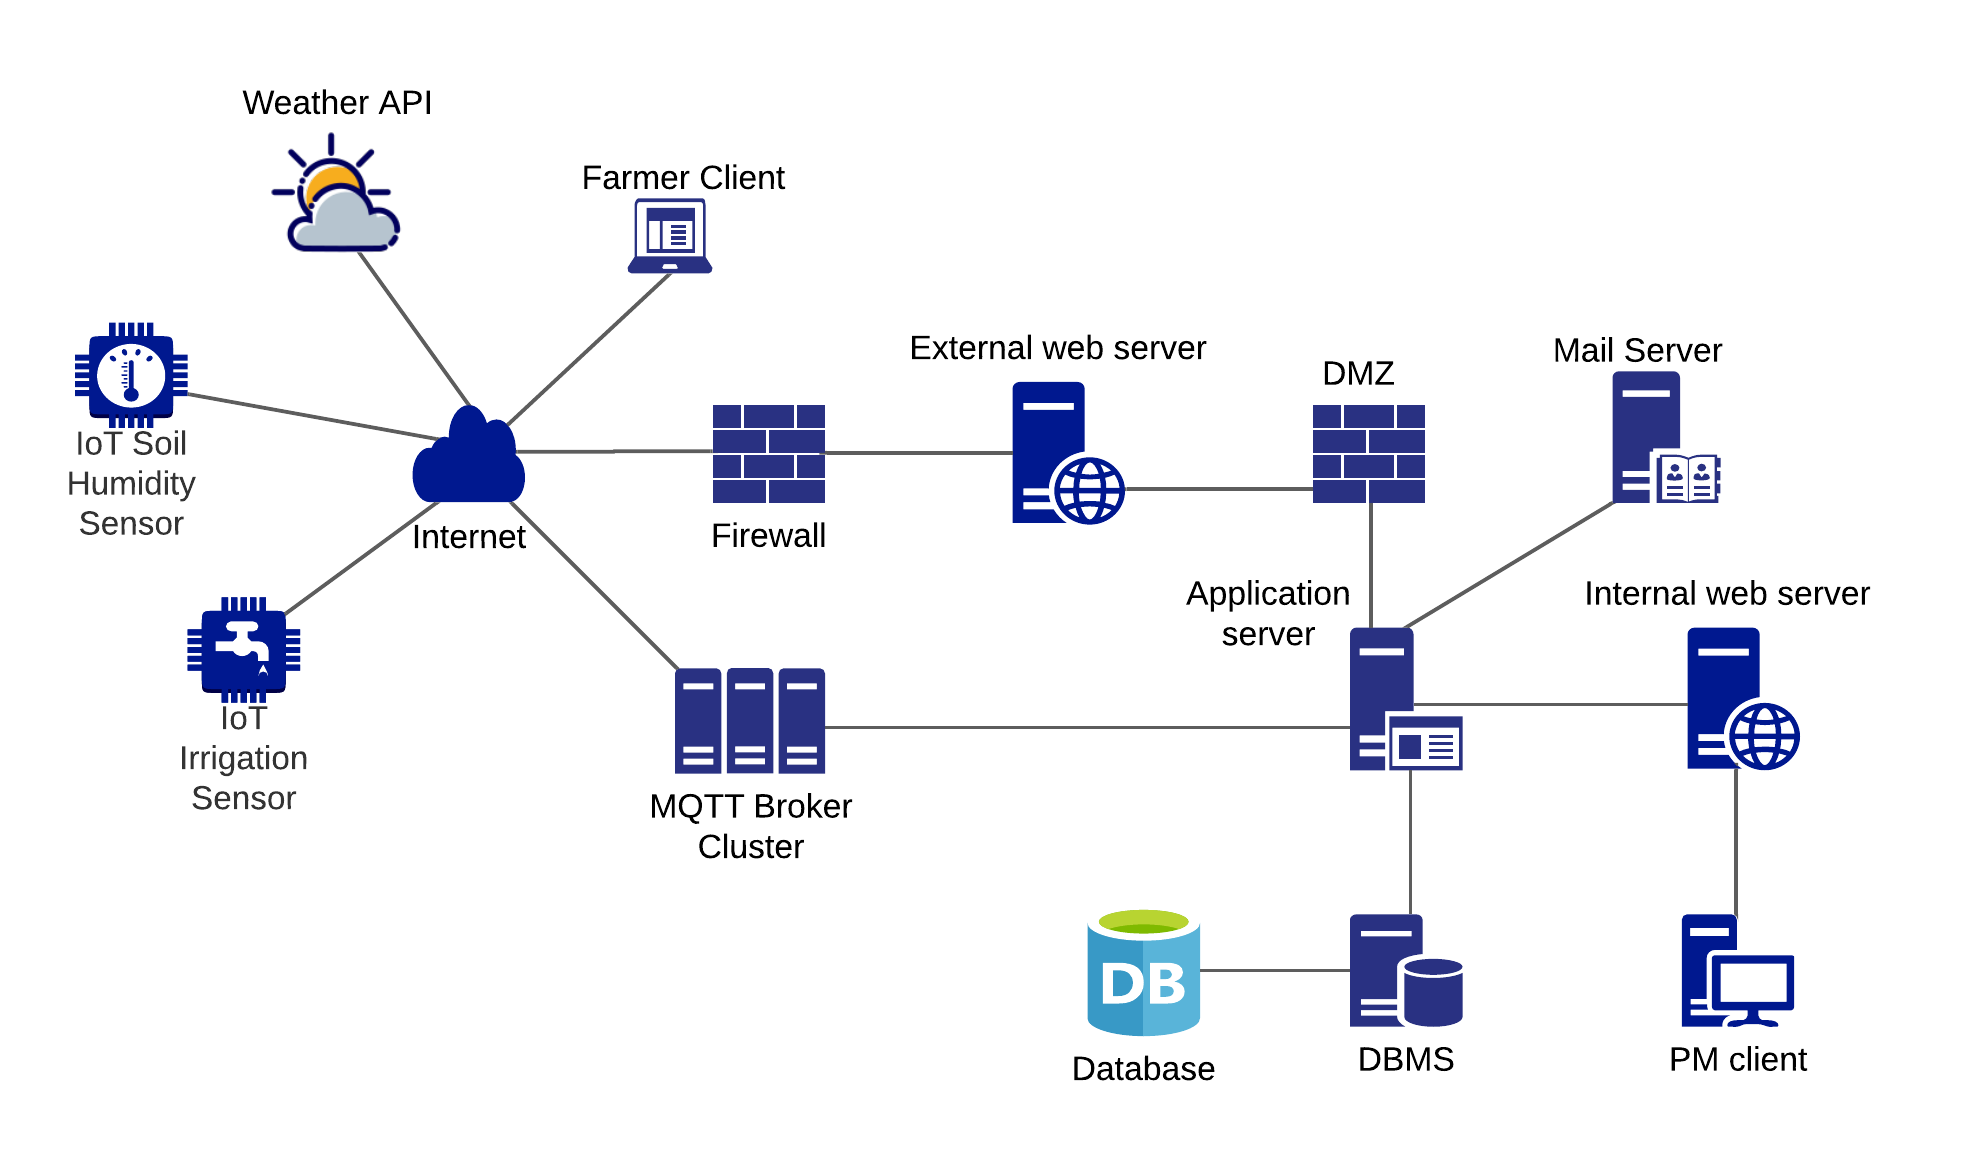
\includegraphics[scale=0.7]{images/overview_architecture.png}
    \caption{System architecture}
    \label{fig:overview}
\end{figure}
The system will be developed from scratch and it will entirely replace the legacy system.\\
The DREAM application is designed with as a three-tier application with web servers, application server, and a database functioning as the three tiers of the application.
The application can be accessed via a webapp provided both to internal and external users. The internal users of the application are the policy maker, that will log into and use the platform
from their workstation, connected to an internal web server. The external users are the farmer, connected to the webapp from their personal computer. This separation between internal and external 
users is meant first and foremost for security requirements, in order not to expose sensitive data to potential risks.\\
Other significant components in the DREAM ecosystem are the IoT sensors, crucial to automatically retrieve and collect data from local farmers and to better evaluate their performances.
IoT sensors are connected via MQTT protocol to a MQTT Broker Cluster which periodically retrieves the data collected by sensors.\\
All the weather informations are taken from the weather forecasting system of Telangana through its APIs.\\
Finally, the application server communicate with a database through a Database Management System.\\
A more detailed description of the components will be given in the following sections.
\subsection{Component view}
\begin{figure}[h]
    \centering
    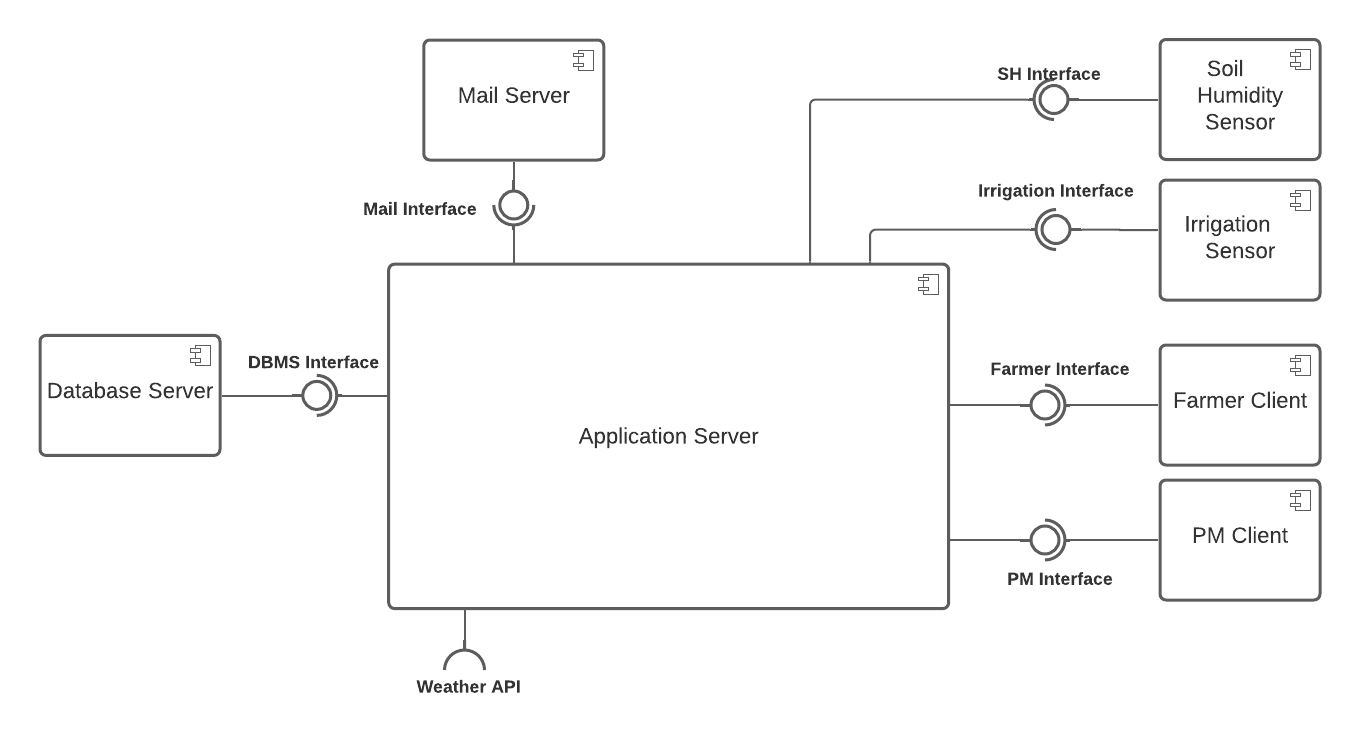
\includegraphics[scale=0.43]{images/hl_component.png}
    \caption{High Level Component Diagram}
    \label{fig:hl_component}
\end{figure}
\begin{itemize}
    \item \textbf{Database server}\\This component is responsible for data management, 
    it provides the interface of the Database Management System to the Application Server, in order to 
    deal with the data management, storing and modification process.
    \item \textbf{Mail server}\\This component allows the Application Server to create and manage email accounts, 
    send and receive email using standard email protocols. The SMTP protocol is used to send messages and handle outgoing mail requests, 
    The IMAP protocol is used to receive messages and to process incoming mail.
    \item \textbf{Application server}\\It is the main component of the system, all the business logic 
    resides in it. This component offers both functionality dedicated to farmers and PMs, 
    interfacing directly with clients. It receives the data entered by the users and sent 
    by the weather forecast system, cross-referencing them and providing for processing, 
    back forwarding and transferring them to the data management system. Its components are 
    described in detail in the following sections.
    \item \textbf{Farmer client}\\It is the component thanks to which the farmers can interface 
    with the Application Server. It represents the web application dedicated to farmers that allows 
    them to access the services of DREAM. This component also receives data from the IoT sensors that 
    monitor the farmer's possessions, making them available to be retrieved from to the Application Server.
    \item \textbf{PM client}\\This is the component thanks to which the Policy Makers can interface 
    with the Application Server. It represents the web application dedicated to them that allows 
    them to take advantage of the services offered by DREAM to monitor and manage agriculture in 
    Telangana. All the functions are accessible thanks to the PM Interface exposed by the Application Server.
    \item \textbf{Soil Humidity and Irrigation sensors}\\
    Sensors for measuring soil humidity and irrigation are 
    internet-connected components responsible for creating and sending data about farmers metrics to the Application Server. 
    They both expose their own interface, through which the Application Server can retrieve the data of interest.
\end{itemize}
\subsubsection{Application Server}
The application server contains the business logic of the application. The following diagram describe its internal structure:
\begin{figure}[h]
    \centering 
    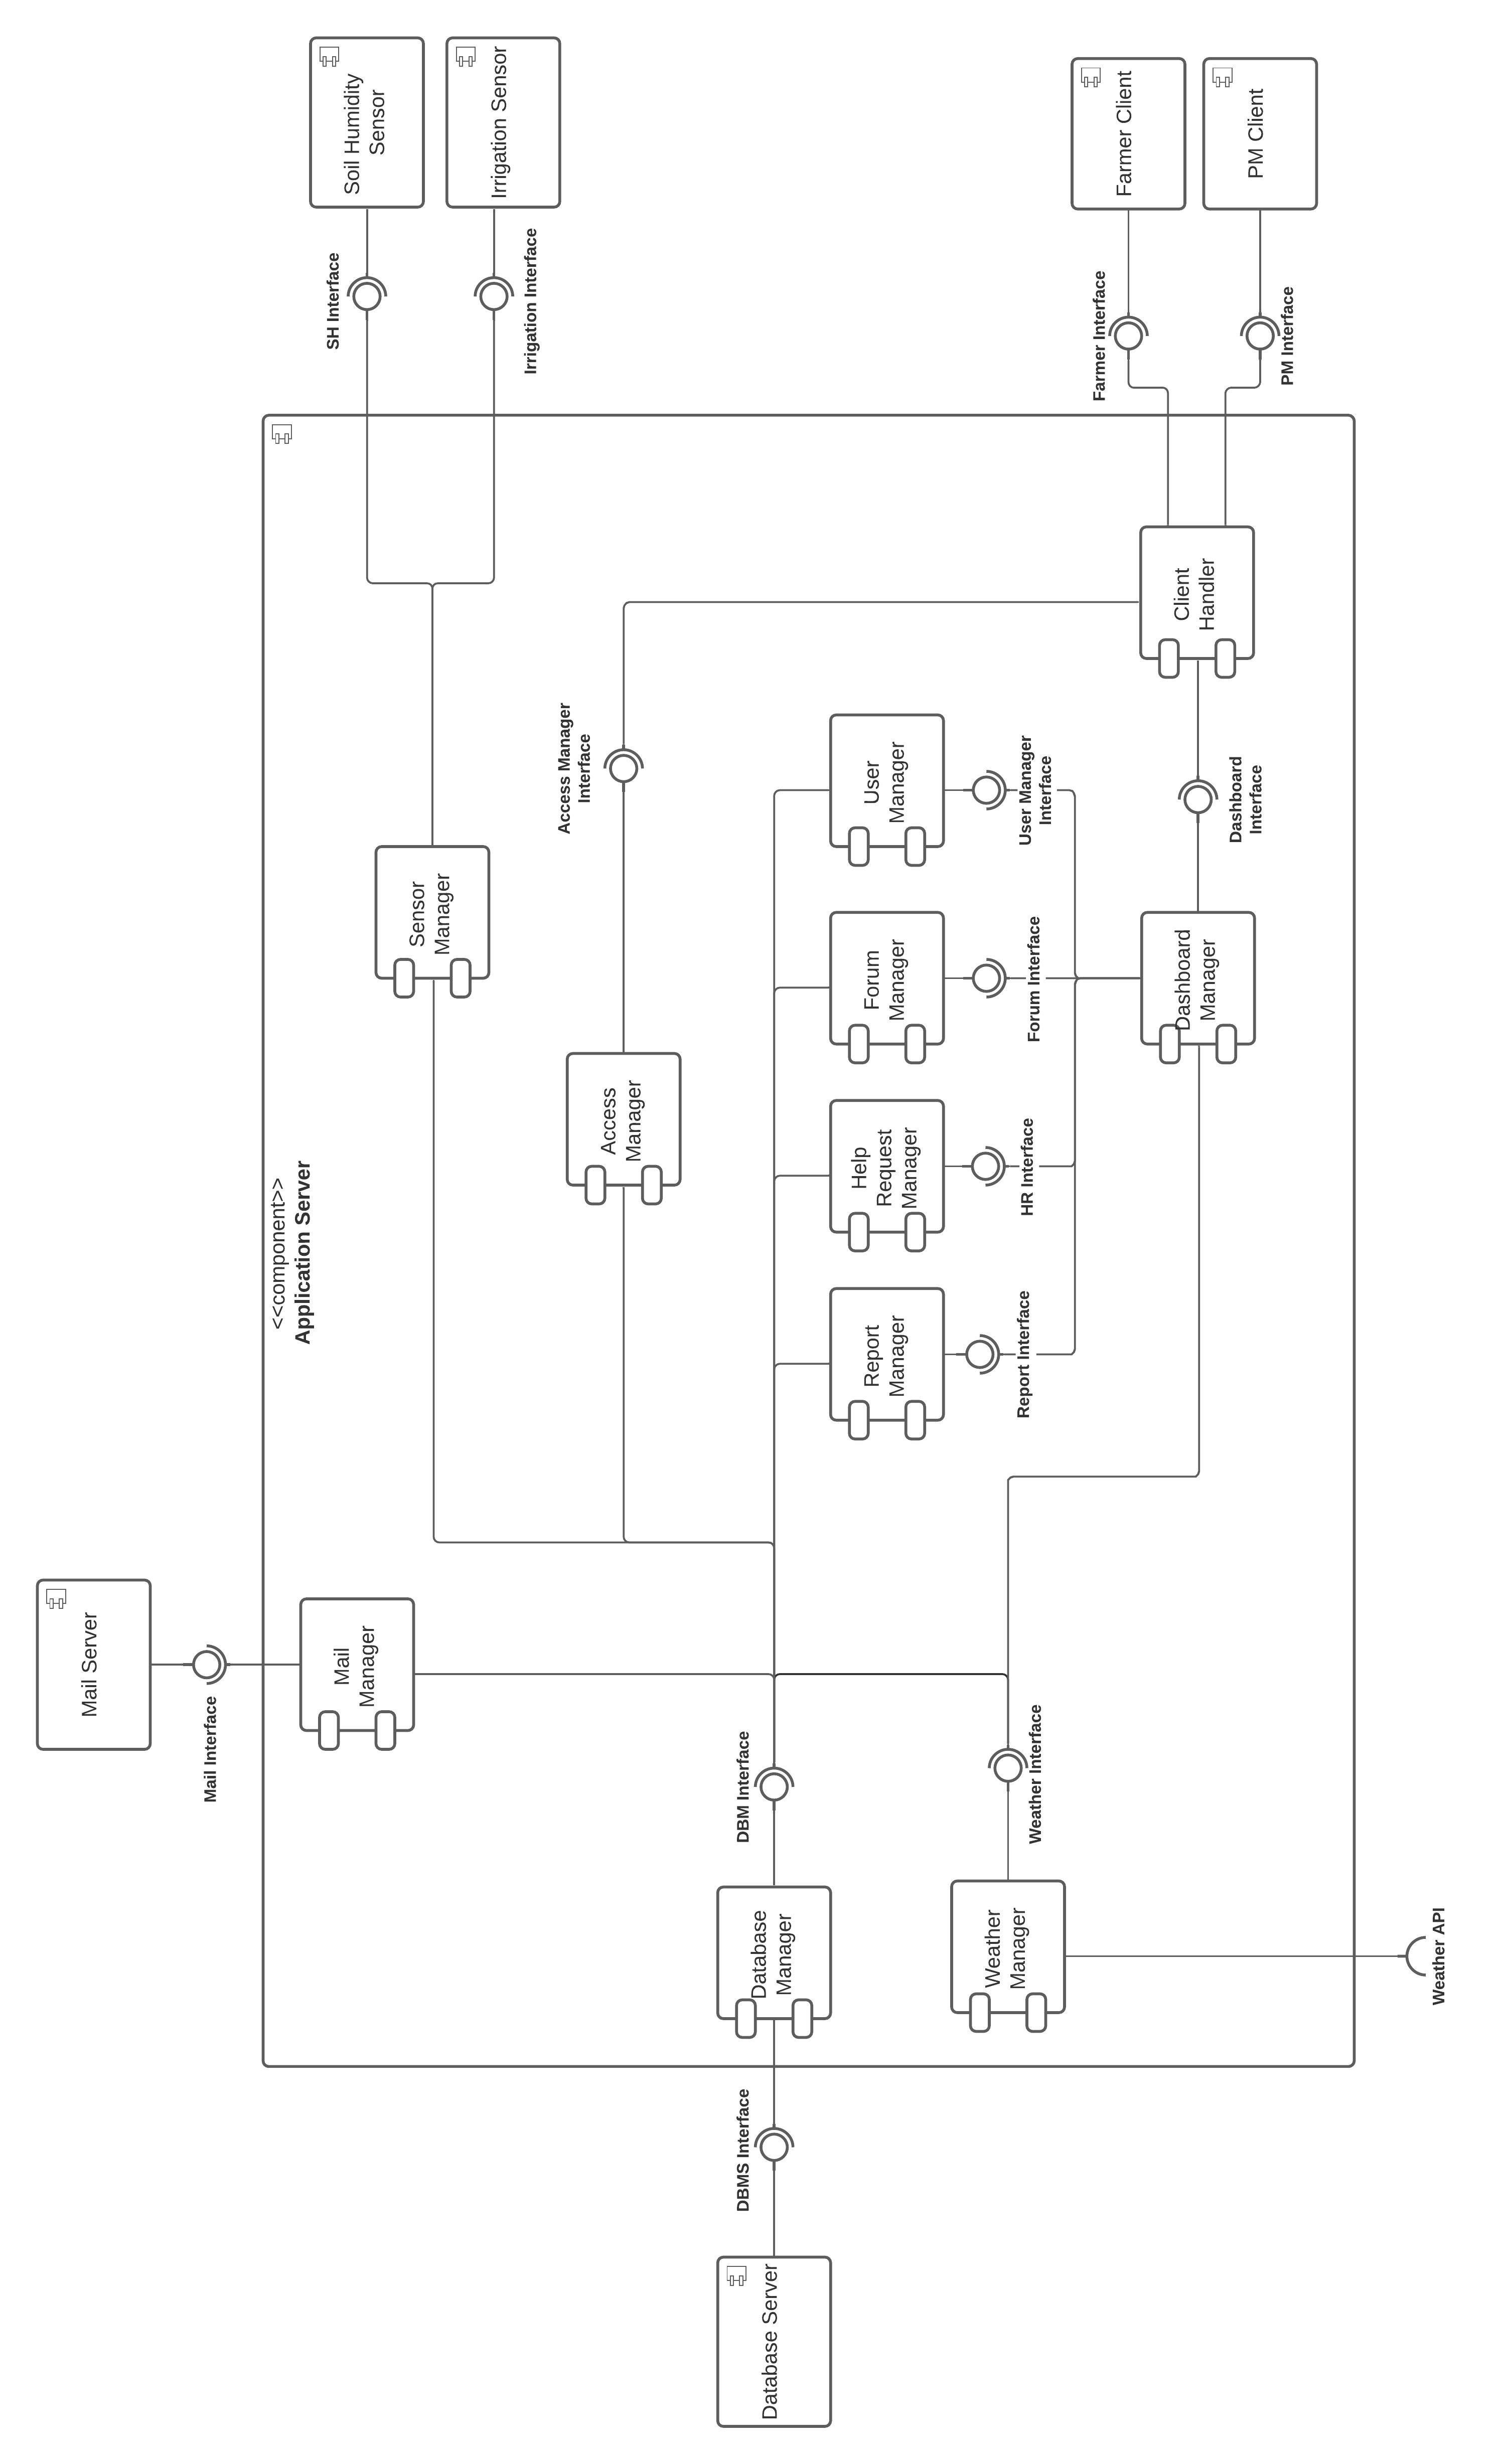
\includegraphics[scale=0.38]{images/app_server_component.png}
    \caption{Application Server Component Diagram}
    \label{fig:app_component}
\end{figure}
The components of the application server are:
\begin{itemize}
    \item \textbf{Database Manager}: deals with management of the data model and data operations, working as a bridge between the physical database 
    and the other components of the server.
    \item \textbf{Mail Manager}: interfaces between the server components and the mail server in order to provide mailing services.
    \item \textbf{Weather Manager}: interfaces between the external weather forecasting API and the other server components.
    \item \textbf{Access Manager}: handles the authentication procedure of the application's users. It is also responsible for the generation of access credentials.
    \item \textbf{Sensor Manager}: handles the communications between the application and the sensors installed in the Telangana territory. Manages the retrieving of 
        collected data from the sensors and its processing and storing procedure.
    \item \textbf{Report Manager}: handles the creation and the visualization of reports.
    \item \textbf{Help Request Manager}: handles the creation, the handling and the visualization of help requests.
    \item \textbf{Forum Manager}: handles forum operations such as creation of threads, answering, visualization and moderation.
    \item \textbf{User Manager}: manages the retrieving of user information from the database.
    \item \textbf{Dashboard Manager}: manages the process of generation of web pages, retrieving the necessary data from the other interfaces, and the handling of user requests. 
        This component will be further analyzed in the following part of the document.
    \item \textbf{Client Handler}: handles clients' connection, interfacing between the application server and the clients.
\end{itemize}
\subsubsection{Client Handler}
Figure \ref{fig:client_handler} describes the internal structure of the Client Handler component. This component receives requests from clients and forwards them to the 
Dashboard Manager or to the Access Manager, accordingly to the type of request. The internal component that is key to this operation is the Request Handler, which unpacks the client request 
and calls the corresponding method provided by the Dashboard Interface or the Access Manager Interface. 
\begin{figure}[h]
    \centering 
    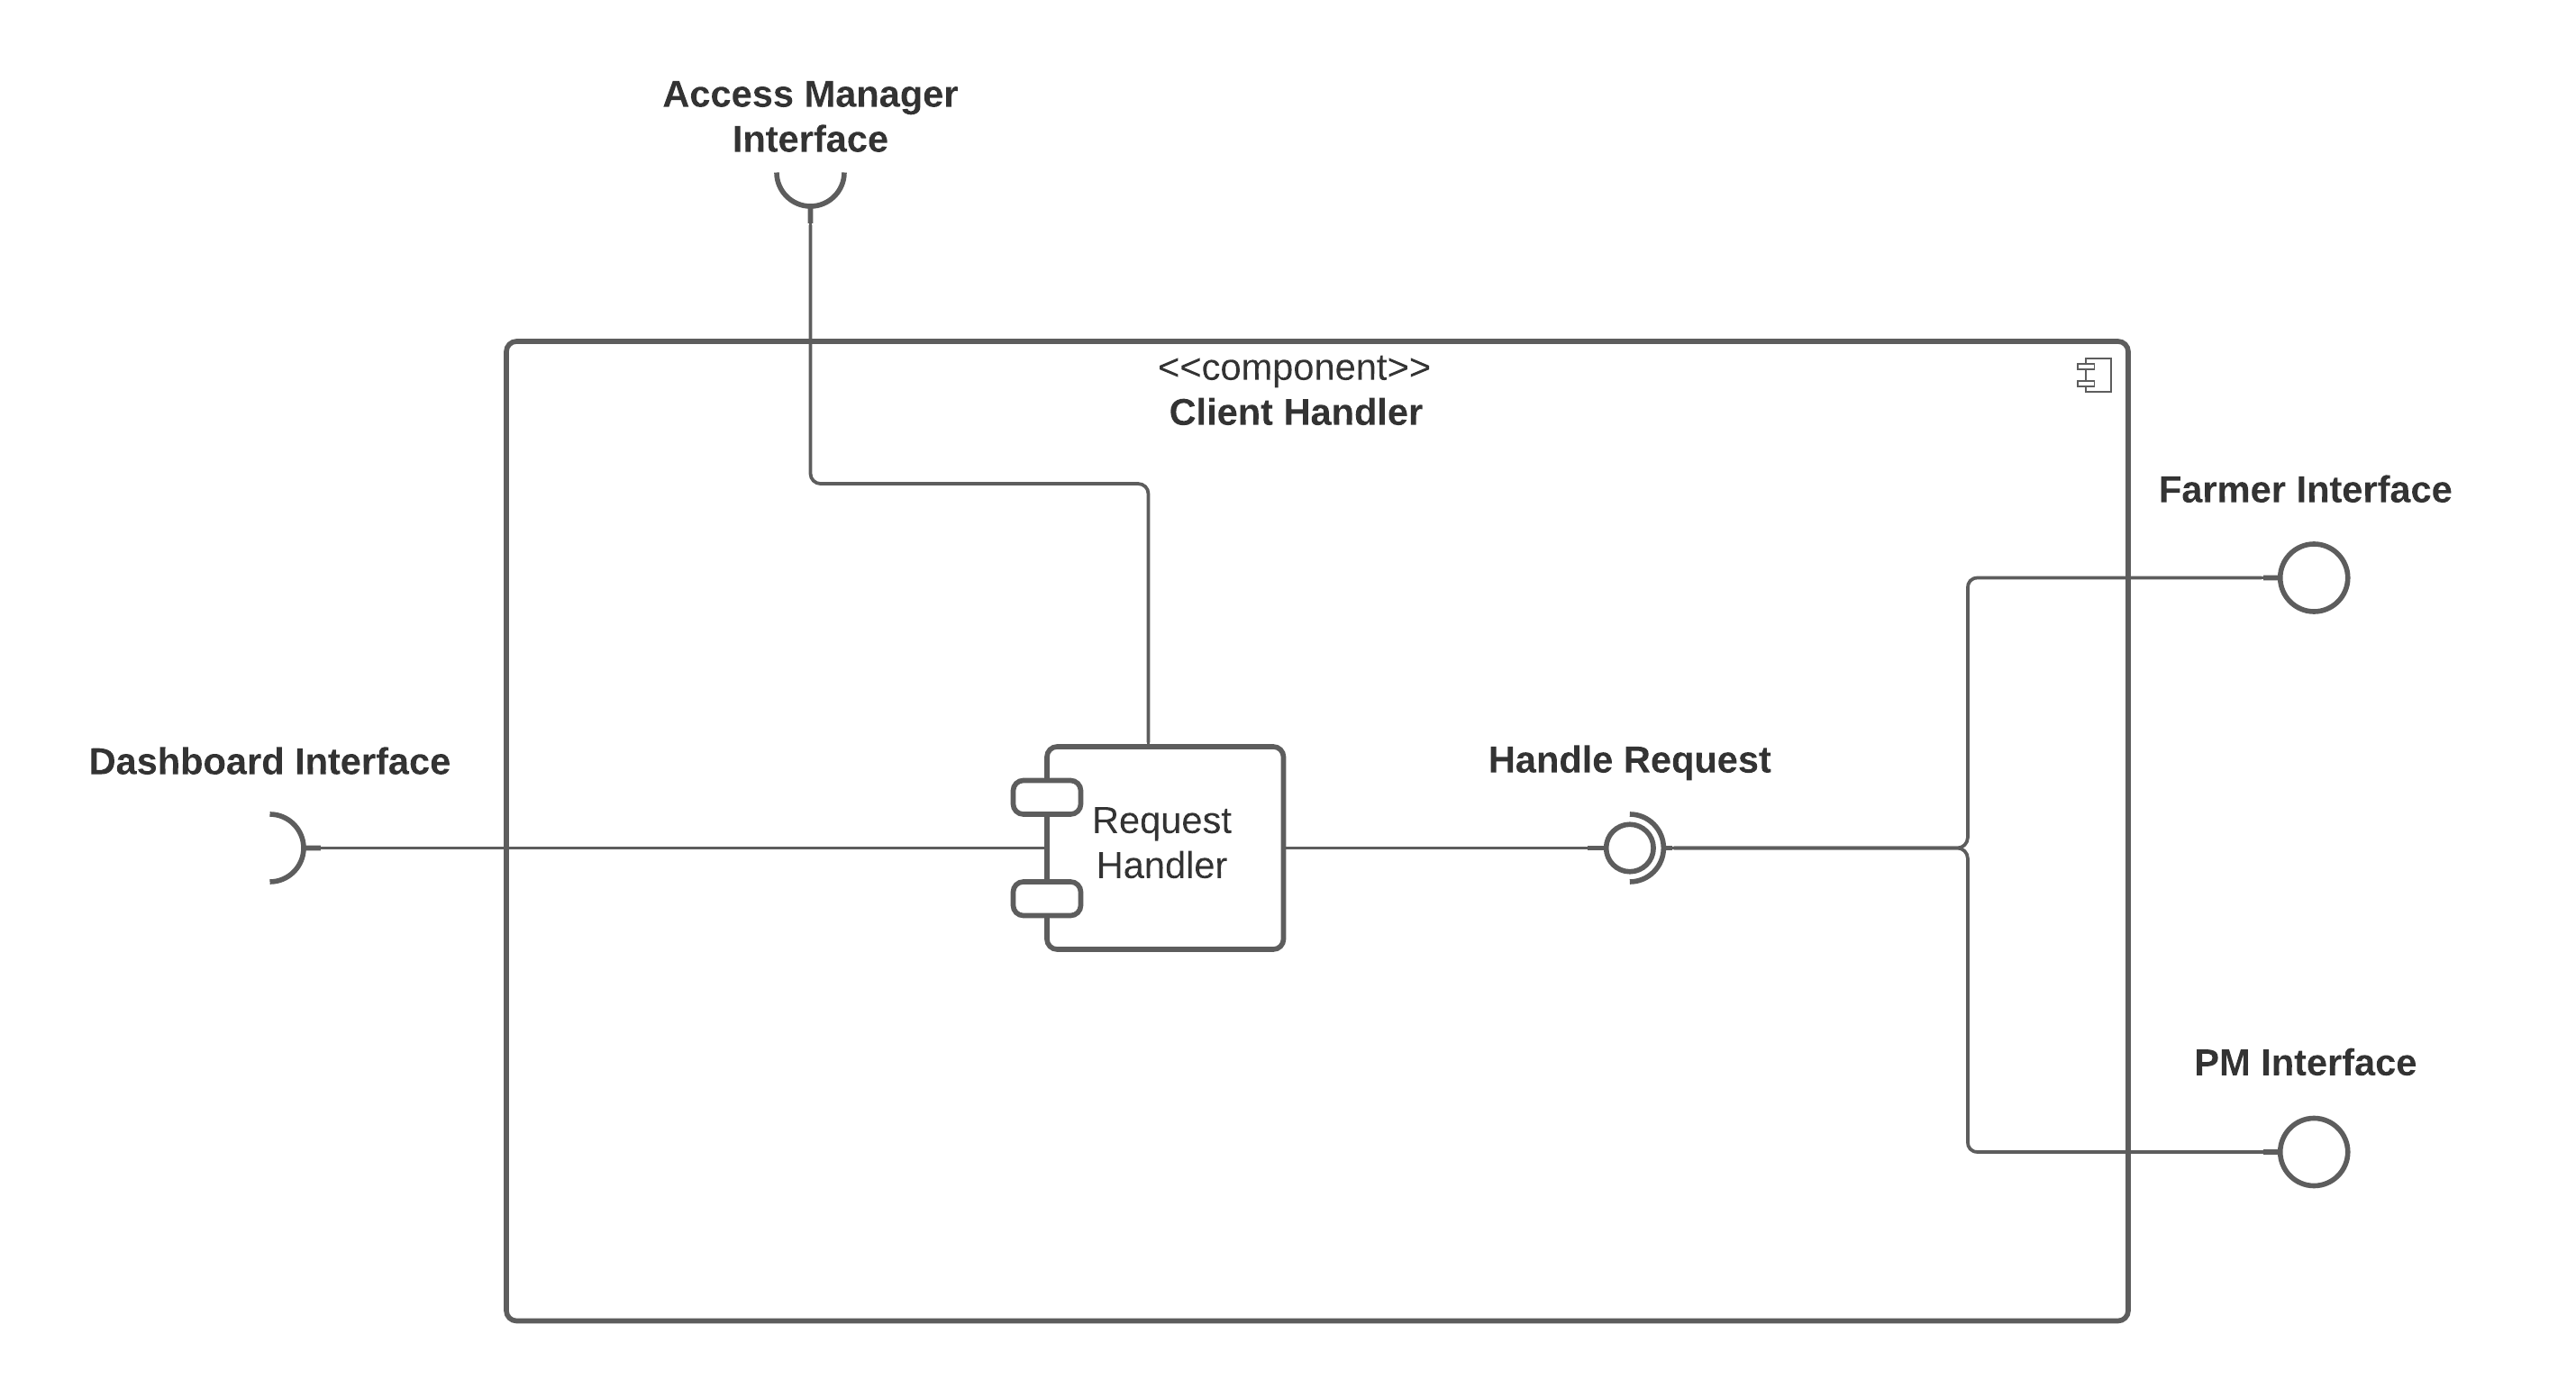
\includegraphics[scale=0.5]{images/clientHandler.png}
    \caption{Client Handler Component Diagram}
    \label{fig:client_handler}
\end{figure}
\subsubsection{Dashboard Manager}
Figure \ref{fig:dashboard_manager} describes the internal structure of the Dashboard Manager component. The Dashboard Manager works as a provider of webpages, forwarded then to 
the user by the Client Handler. Since each webpage is dinamically built by fetching data from the model, this component is interfaced with the various controller components such as Report and Help Request Managers through
their external interfaces. Once a webpage is requested through the Dashboard Interface, the Dashboard Manager internal components proceed to build the webpage by making requests to various components
and once the page has been built it is returned from the interface.
\begin{figure}[h]
    \centering 
    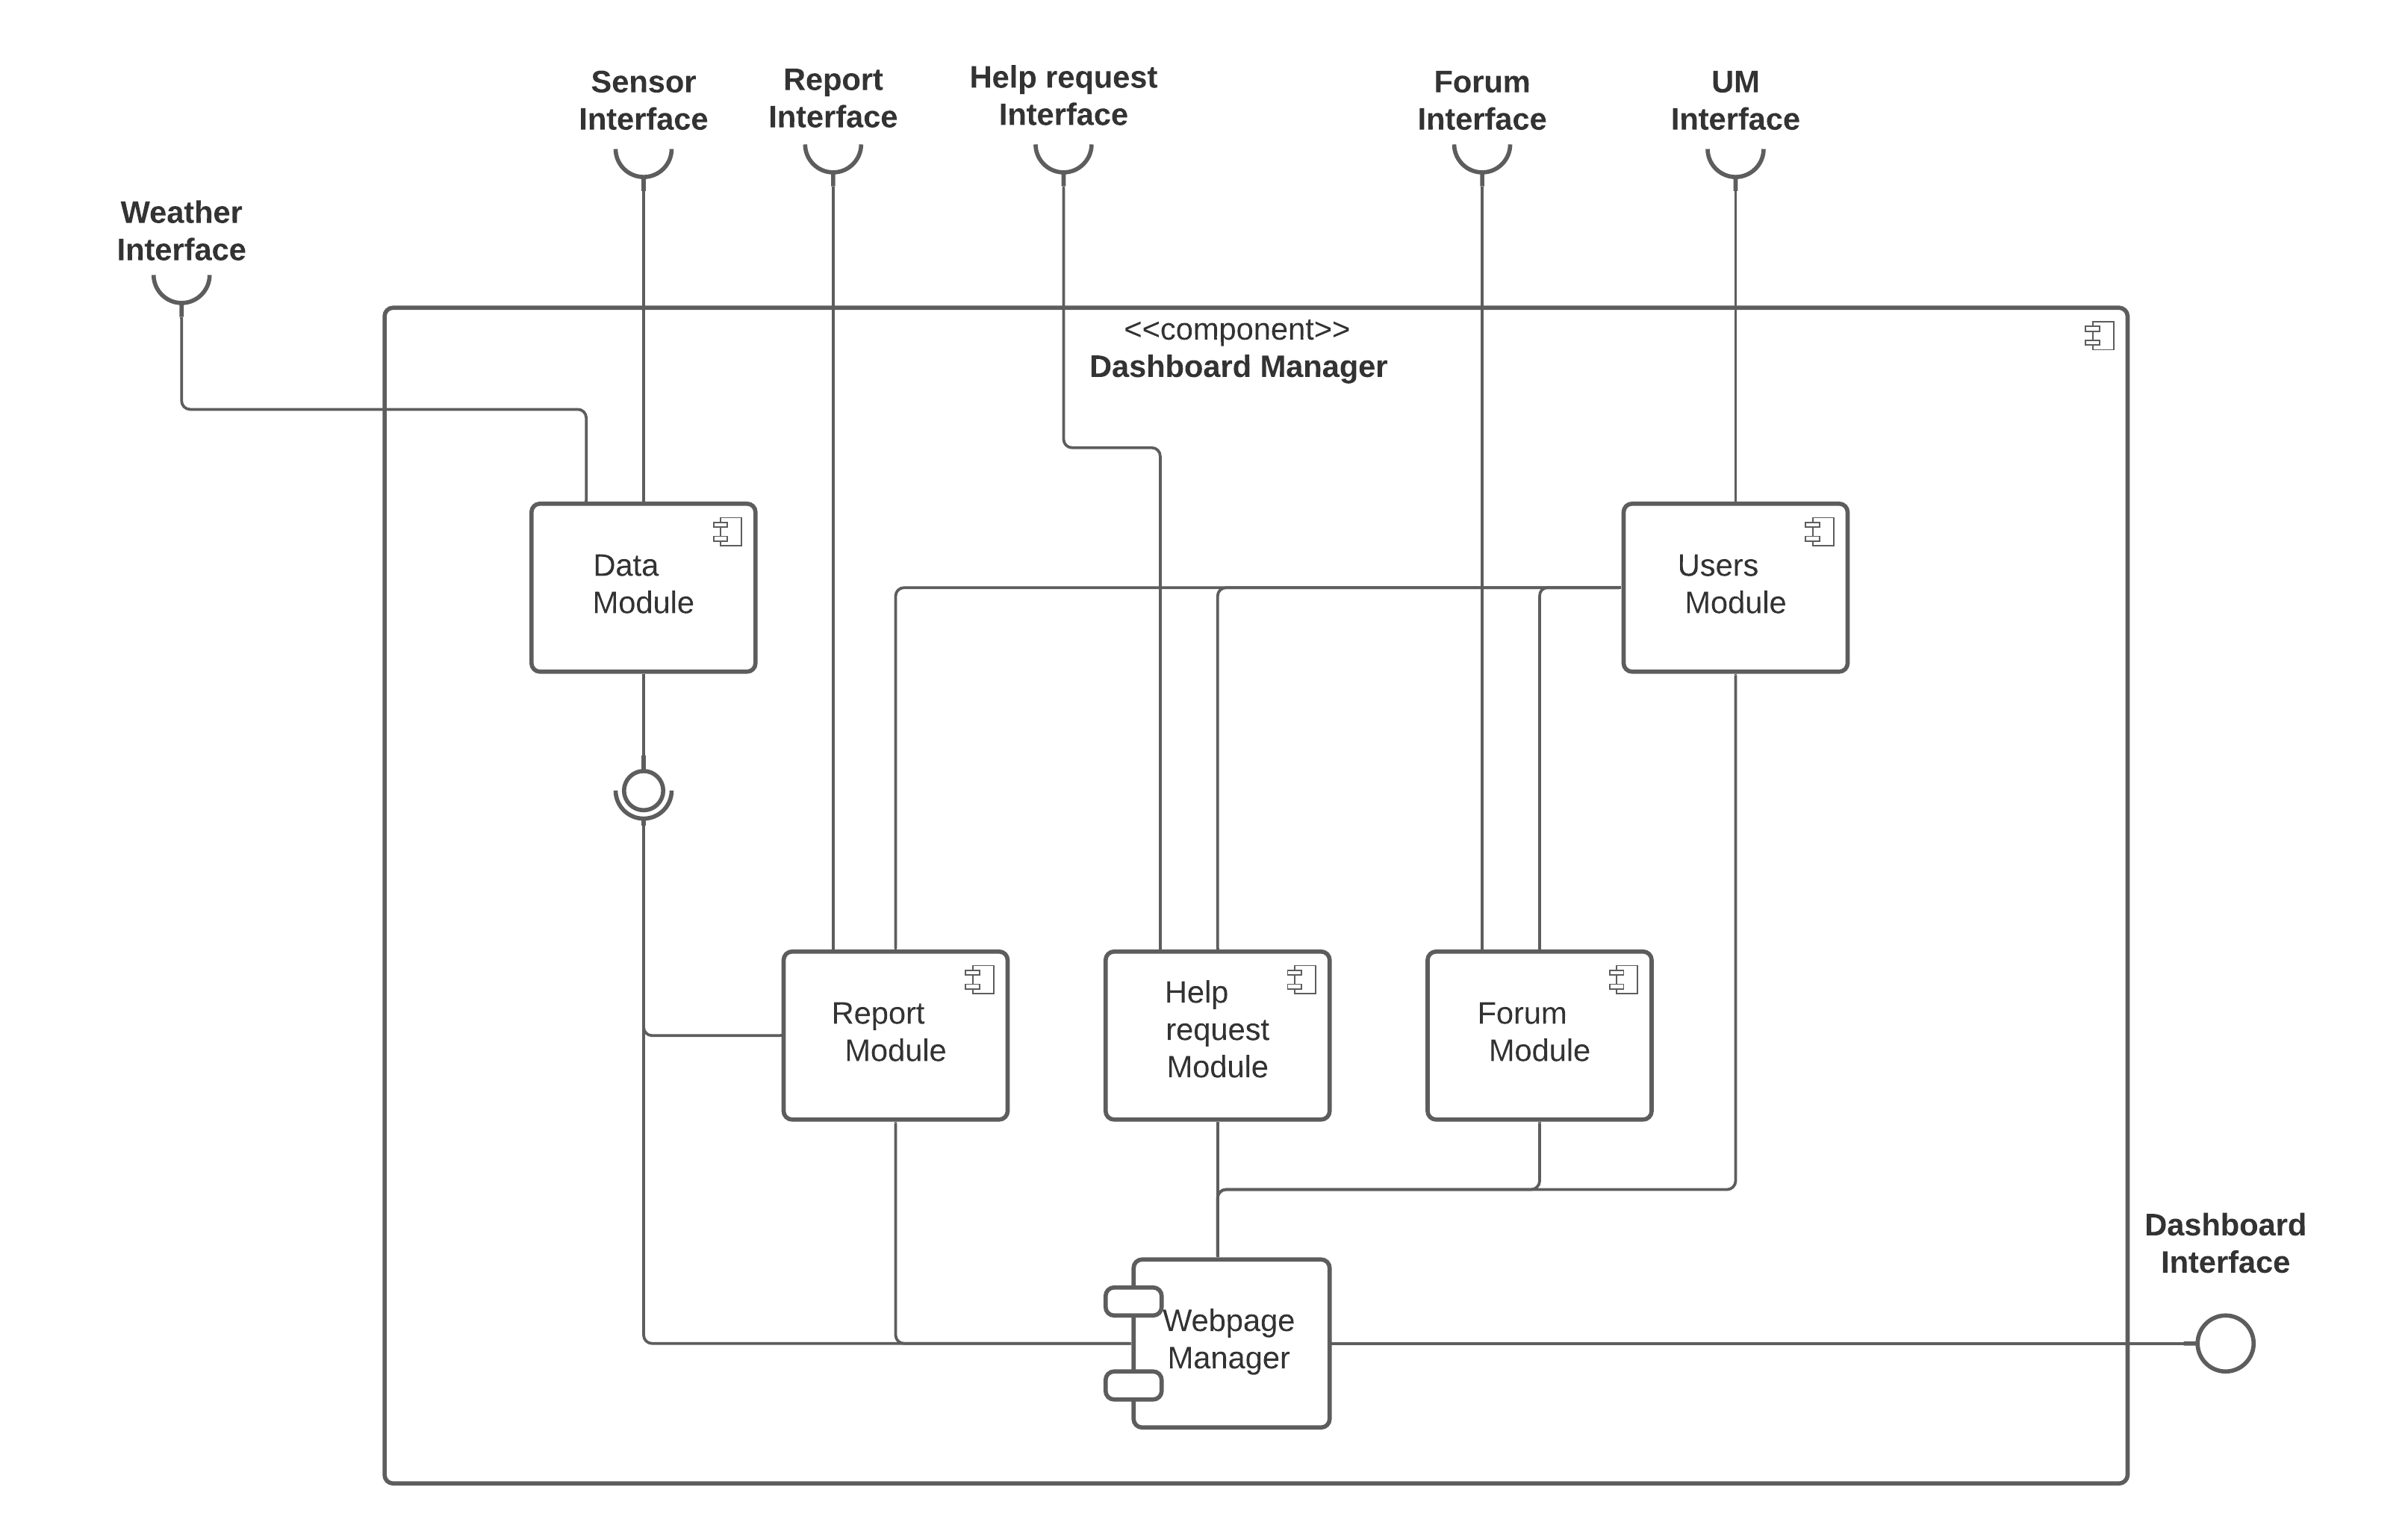
\includegraphics[scale=0.4]{images/dashboardManager.png}
    \caption{Dashboard Manager Component Diagram}
    \label{fig:dashboard_manager}
\end{figure}
\subsection{Deployment view}
Figure \ref{fig:deployment} describes the deployment components of the application. The system is implemented as a three-tier architecture,
a standard software application architecture dividing the application into three logical and physical tiers that is present in most of client-server applications.
The three tiers of the architecture consist in:
\begin{itemize}
    \item \textbf{Tier 1: Presentation tier}: the presentation tier comprises the user interfaces and the communication layers, providing services to display data to end users and allowing
        them to interact with the application. In the DREAM deployment, this tier is composed of a web server installed on a dedicated server instance with Apache TomEE 8, responsible for the interaction with end users, and an MQTT broker that periodically 
        interacts with the sensors installed on a dedicated broker server.
    \item \textbf{Tier 2: Application tier}: the application tier implements the business logic of the application, providing the necessary back-end services.
        This tier collects information from the presentation tier and interacts with the data tier through CRUD operations. The DREAM application server is installed on a dedicated 
        server instance, running a Java Virtual Machine.
    \item \textbf{Tier 3: Data tier}: the data management tier provides database services accessed by the application tier and the presentation tier. The DREAM data management tier is installed on a dedicated
        MySQL server and accessed via JDBC and JPA.
\end{itemize}
\begin{figure}[h]
    \centering
    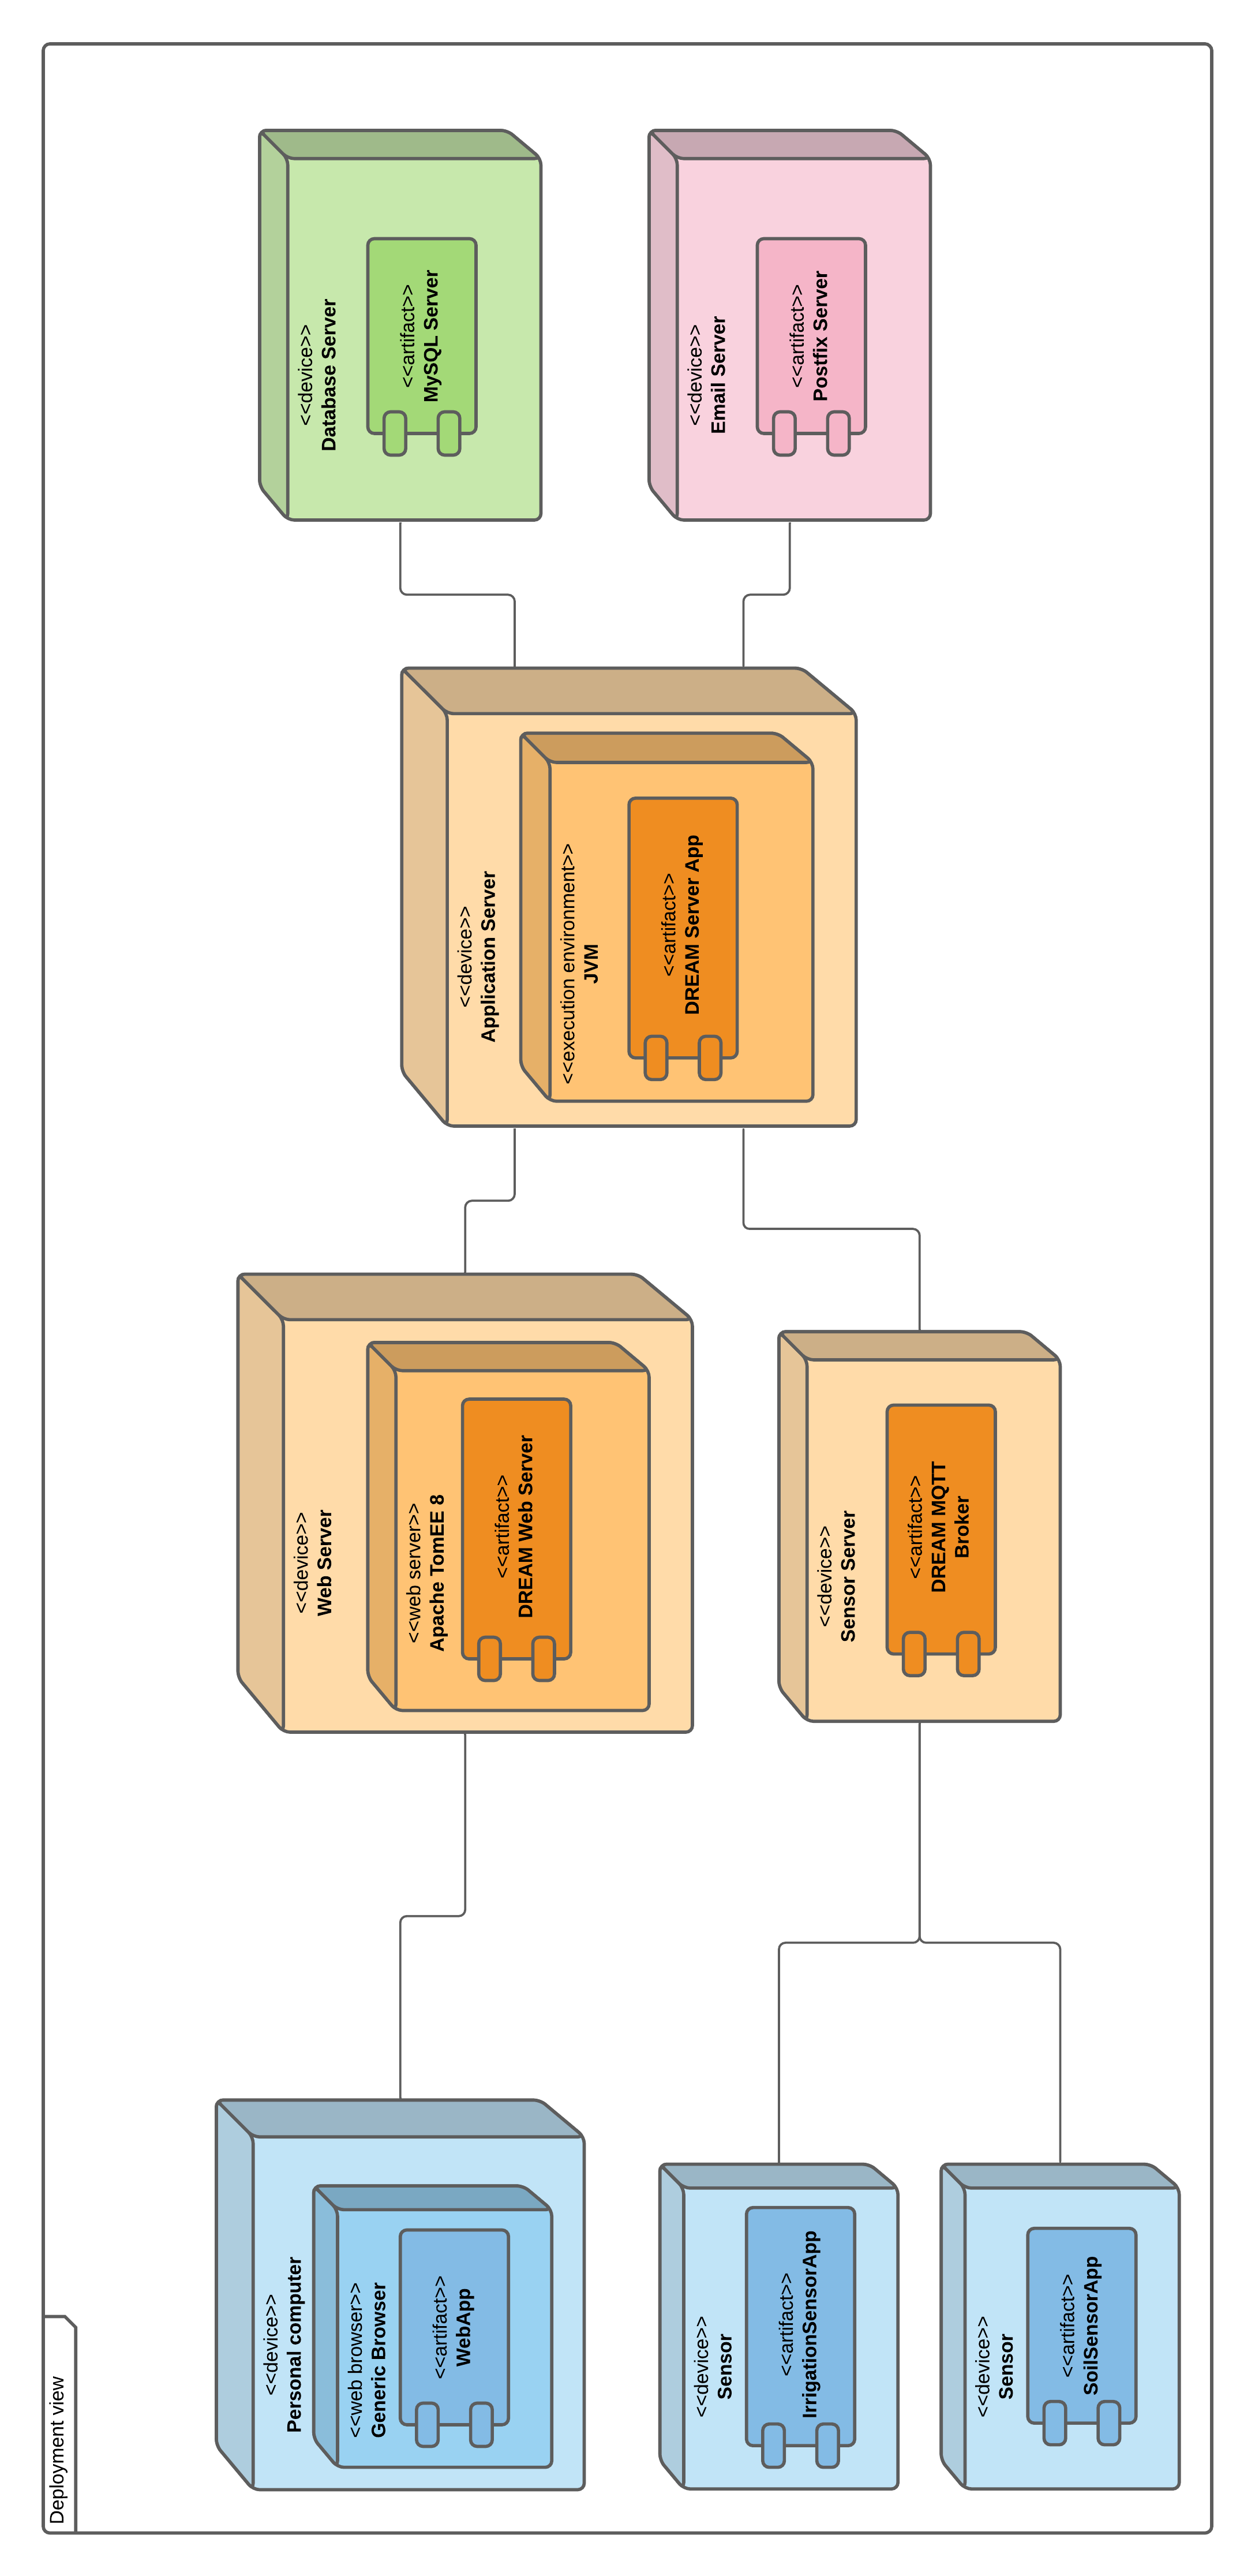
\includegraphics[scale=0.43]{images/deployment.png}
    \caption{Deployment Diagram}
    \label{fig:deployment}
\end{figure}
\subsection{Runtime view}
This section aims to describe the interactions between components and their interfaces at runtime, detailing some crucial operations such as login and report insertion.
It should be noted that these diagrams are meant to give an idea of the behaviour of the system and to provide a blueprint for the implementation of these processes. 
The methods used in the diagrams are the ones provided by each component's interface. Internal methods of a component are only shown if particularly relevant to the operation.
\subsubsection{Registration}
Figure \ref{fig:r_registration} shows the registration procedure for both farmers and policy makers. These procedures differs in some points but the overall system behaviour
is similar. For what concerns the farmer registration process, it begins with a request from the policy maker handled by the Access Manager: new credentials are generated, stored into 
the database and sent via e-mail by the Mail Manager component to the farmer. The policy maker registration process is almost the same, with the only difference being that the 
registration procedure is started by a system admin, requesting directly to the Access Manager to generate credentials for the PM. The generated credentials are then stored in the DB and
sent via e-mail to the policy maker.
\begin{figure}[h]
    \centering
    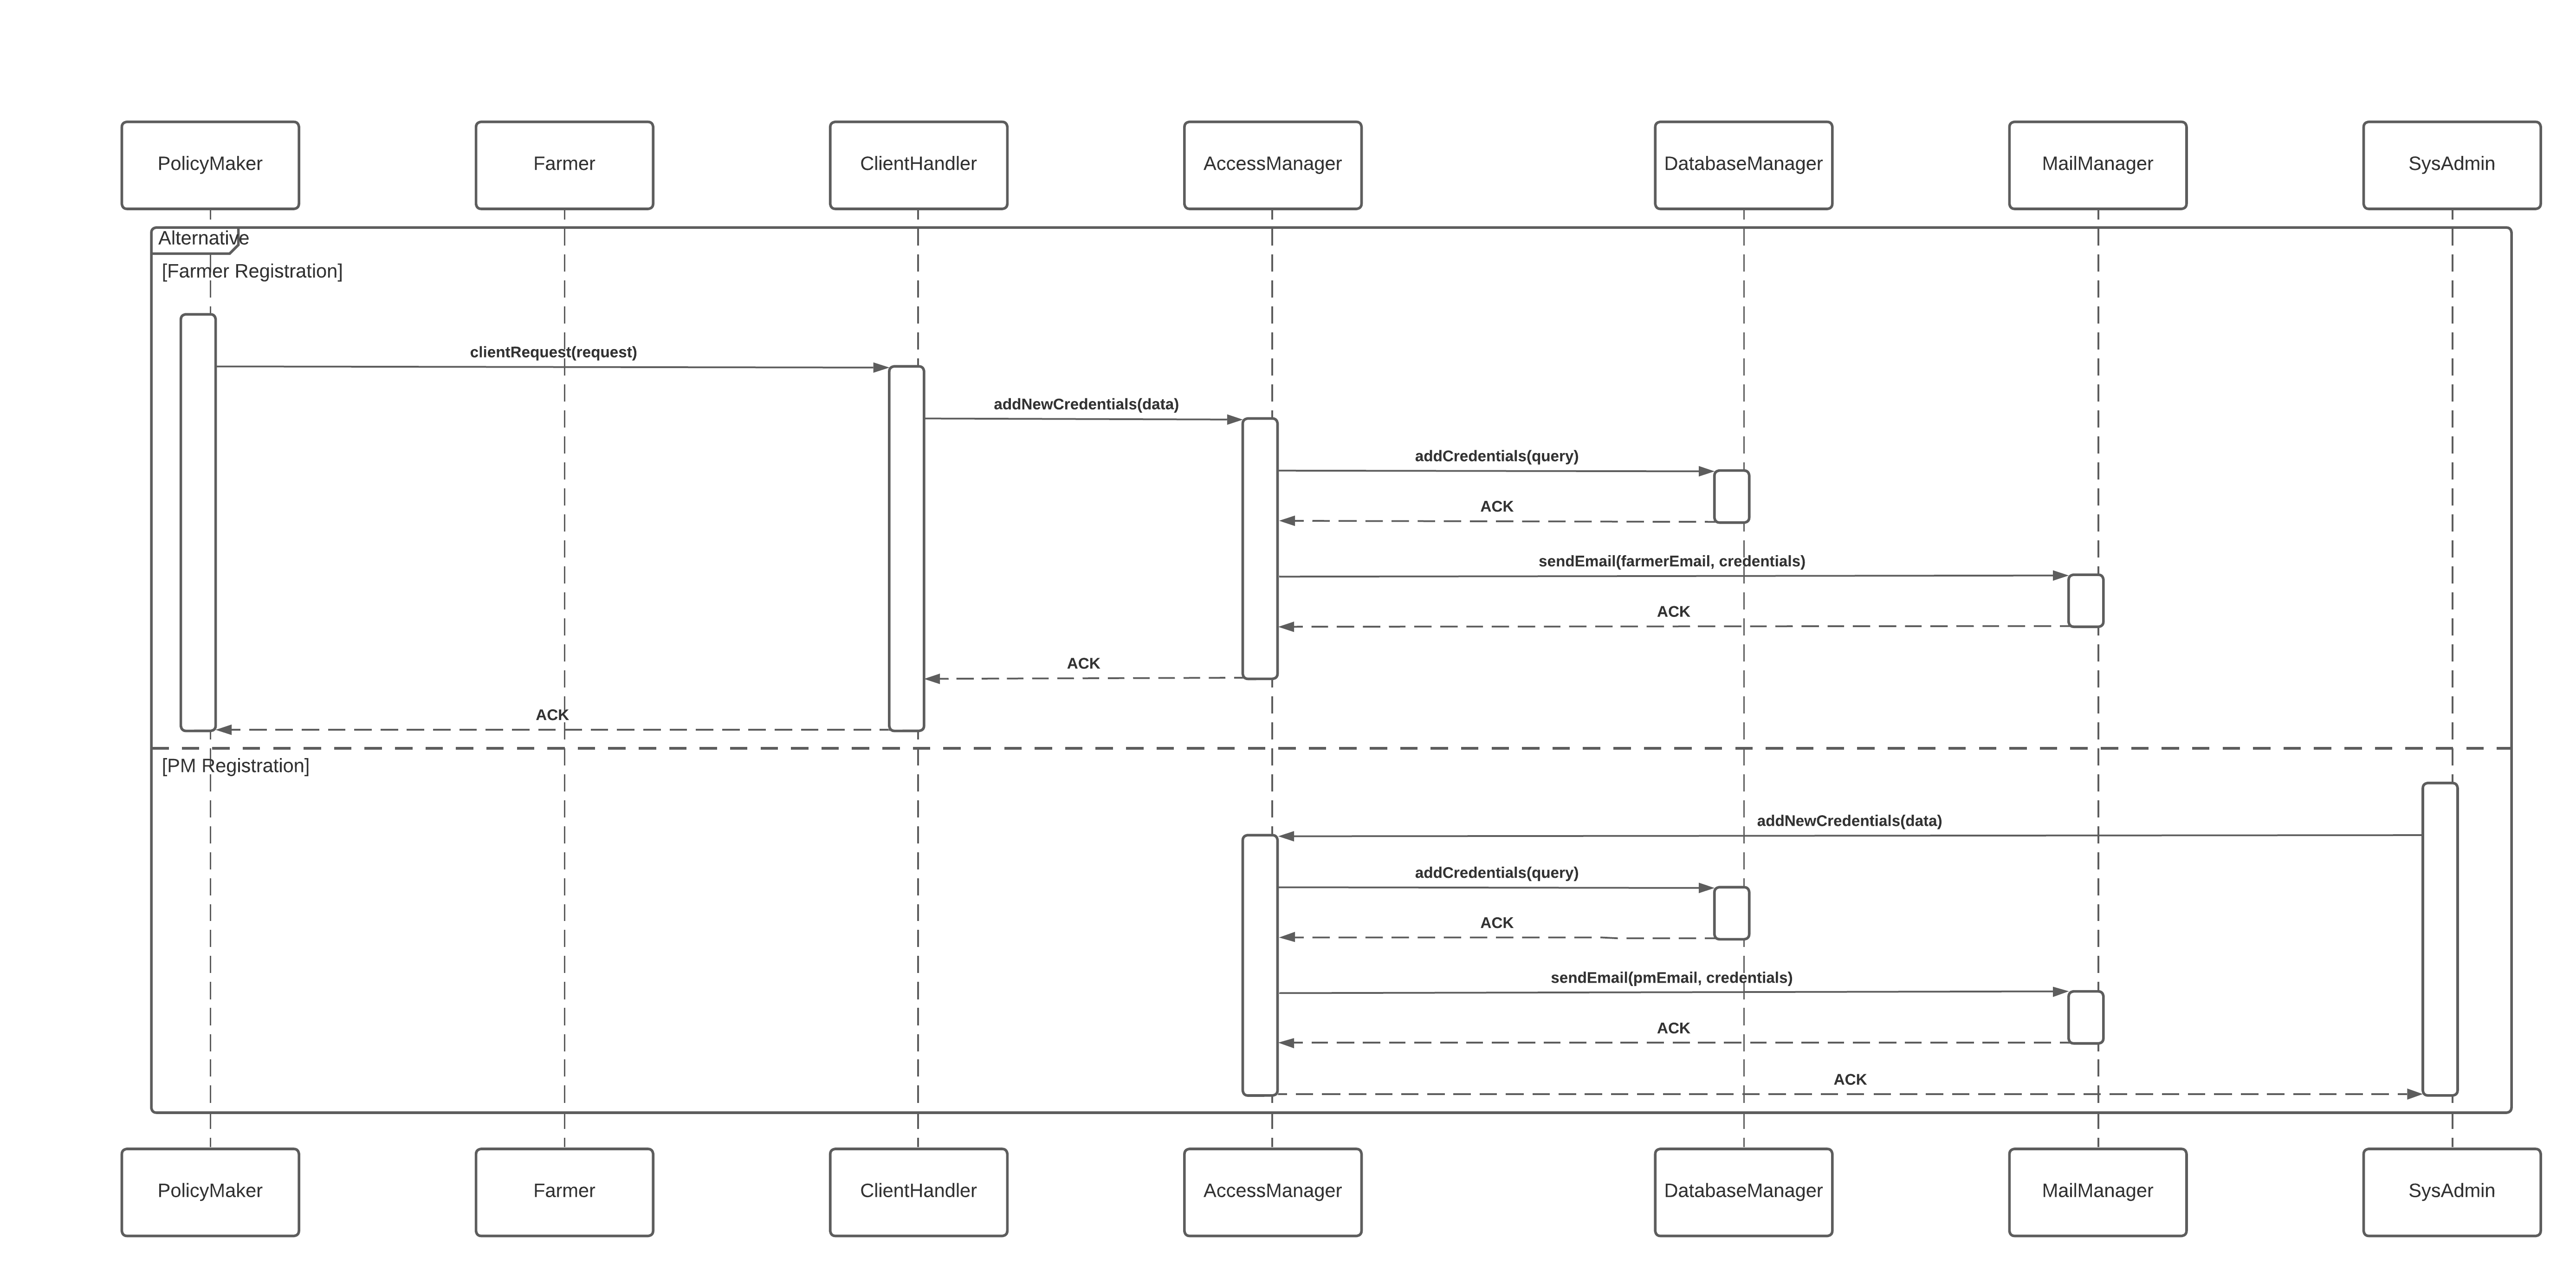
\includegraphics[scale=0.25]{images/rv/registration.png}
    \caption{Registration runtime diagram}
    \label{fig:r_registration}
\end{figure}
\subsubsection{Login}
Figure \ref{fig:r_login} describes the login procedure: the first request to the system is to get the login page, generated by the Dashboard Manager. Once the client has been provided
with the page, it enters his login credentials and the login request is then forwarded to the Access Manager, that verifies the credentials through a DB query and returns the outcome of the request:
if the credentials are correct, the user is redirected to his homepage, otherwise the login page gets newly displayed, this time with an error message.
\begin{figure}[h]
    \centering
    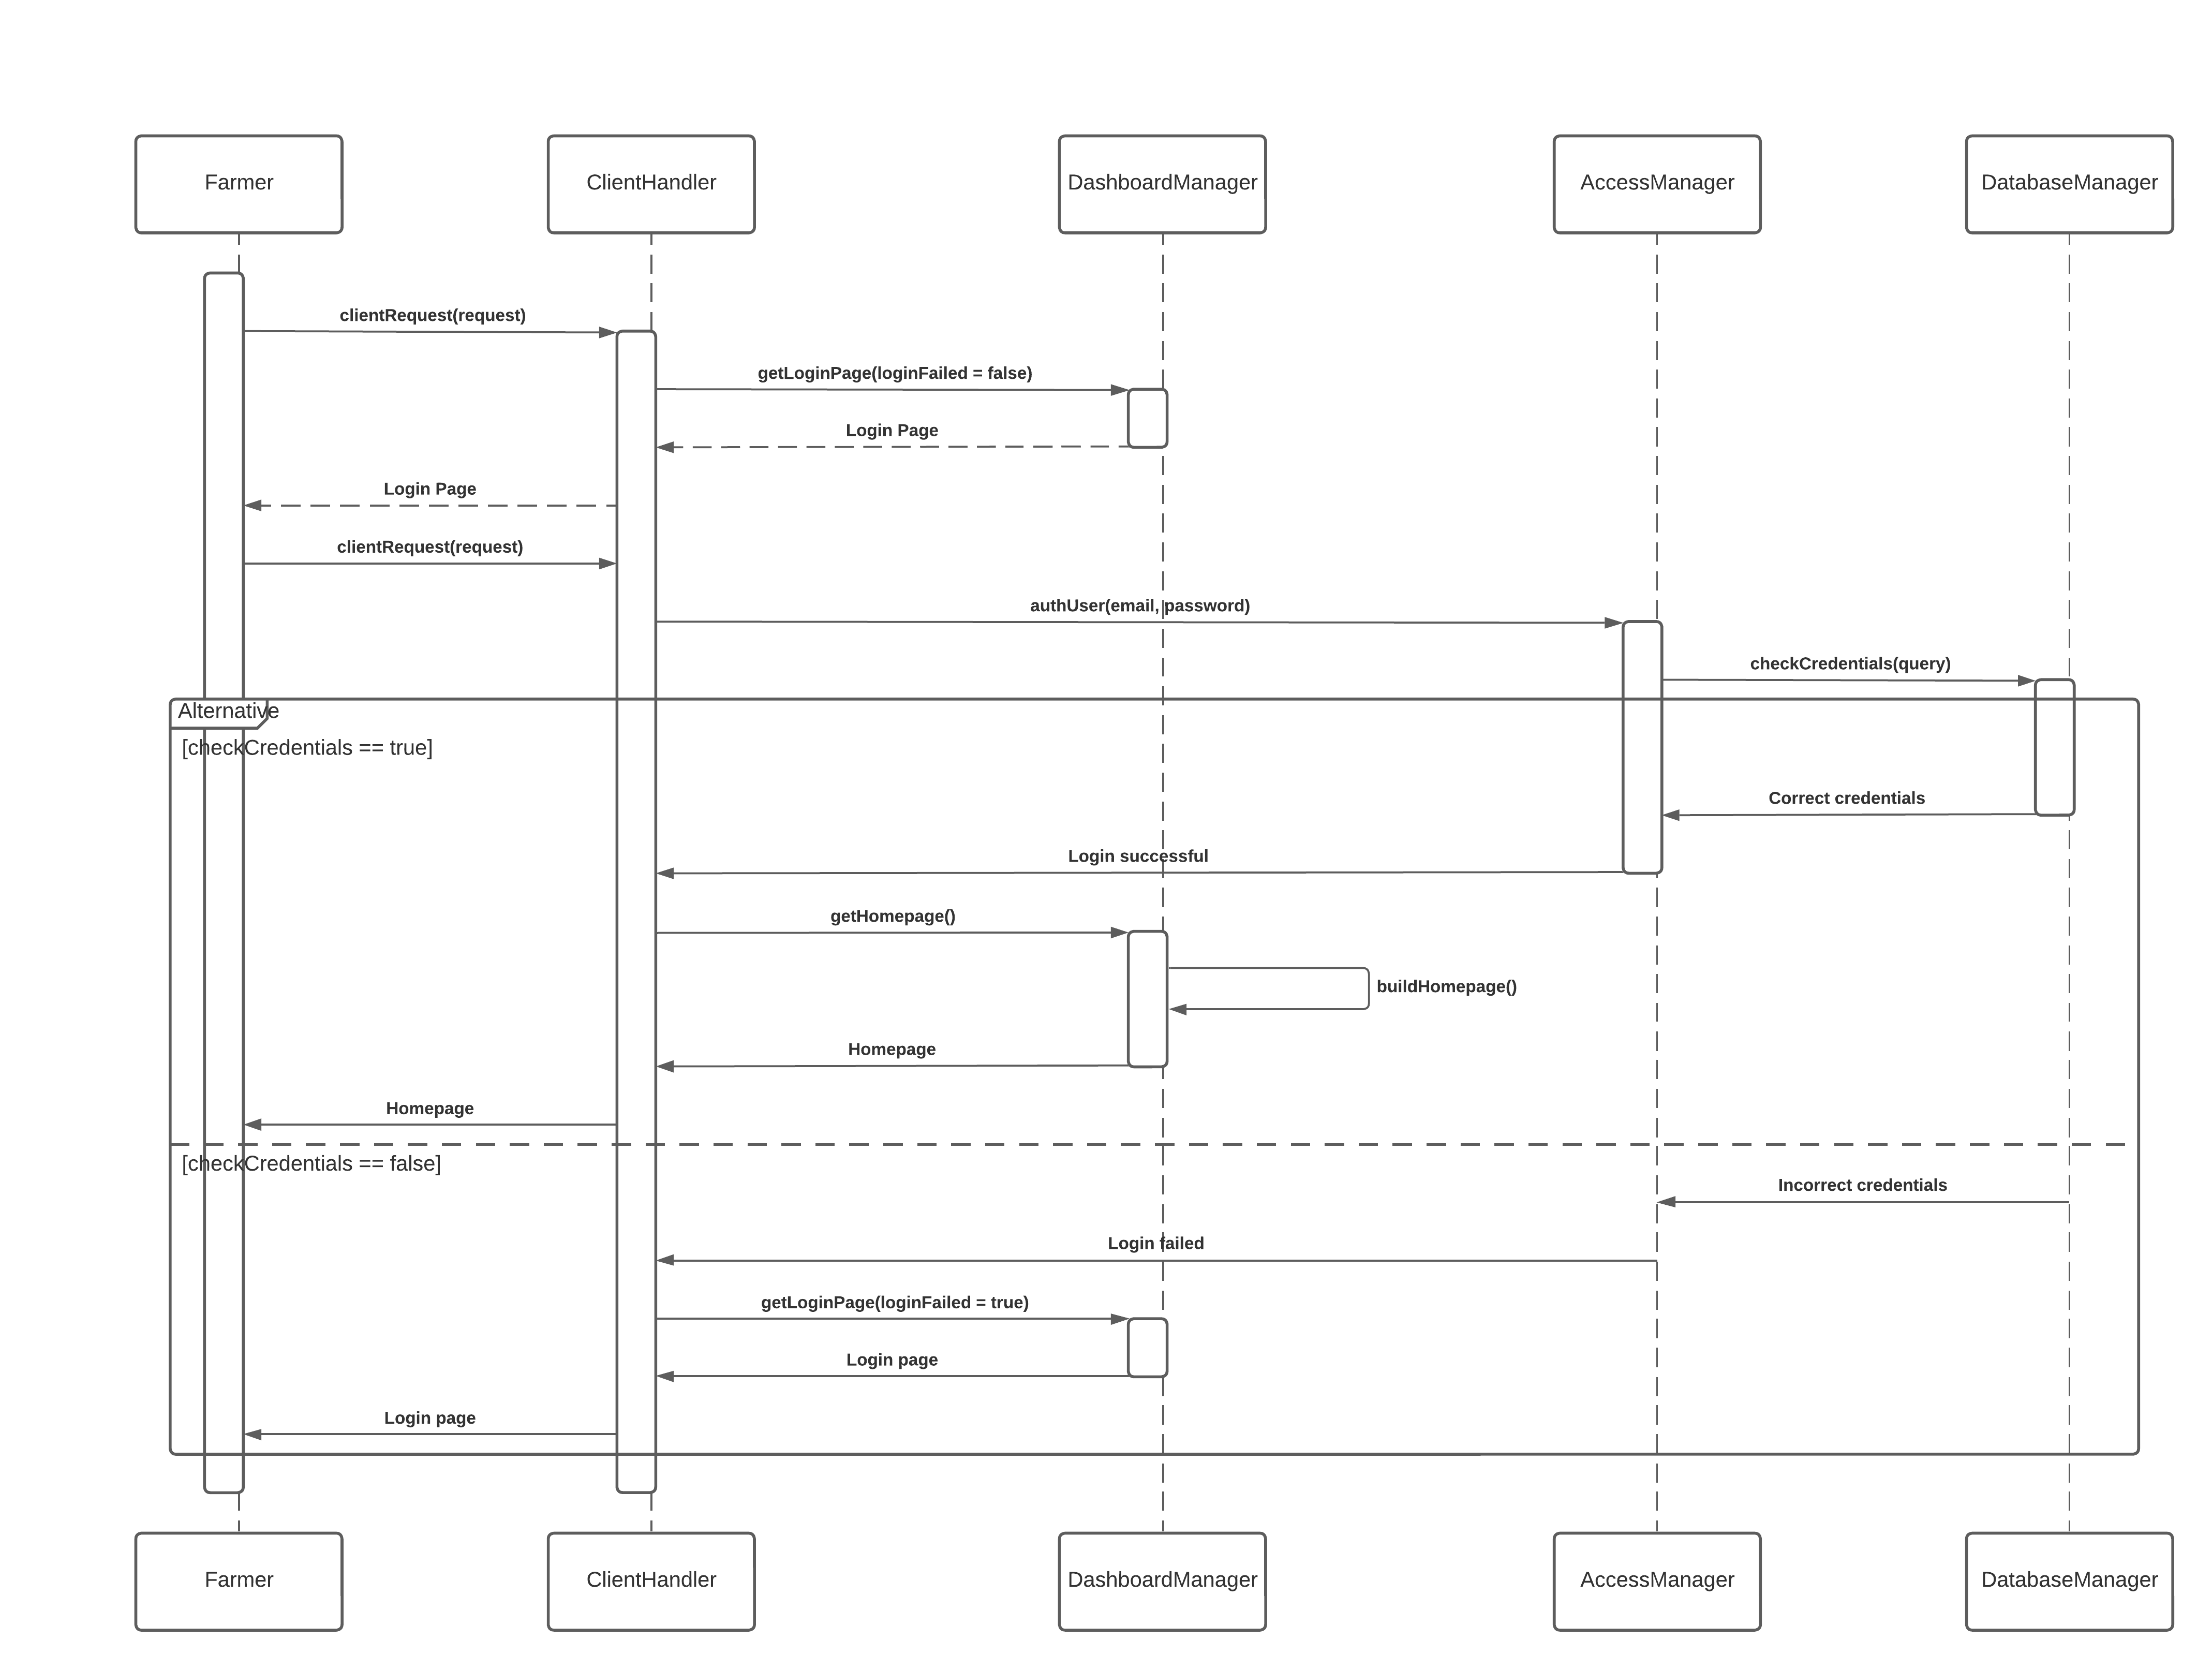
\includegraphics[scale=0.3]{images/rv/login.png}
    \caption{Login runtime diagram}
    \label{fig:r_login}
\end{figure}
\subsubsection{Report insertion}
In Figure \ref{fig:r_report} is described the report insertion procedure. Such as almost every other process, it starts with a request to the Dashboard Manager to get
the webpage containing the form to insert a report. Once the user has compiled such form, the report is submitted and handled by the Report Manager. In this phase sensor data 
and weather data are retrieved from the database through the respective Sensor and Weather Managers and, through the crossData() operation, are binded to the farmer's report.
Once this operation succeeds, the report is stored into the database via the Database Manager and the user is acknowledged of the success of the operation.
\begin{figure}[h]
    \centering
    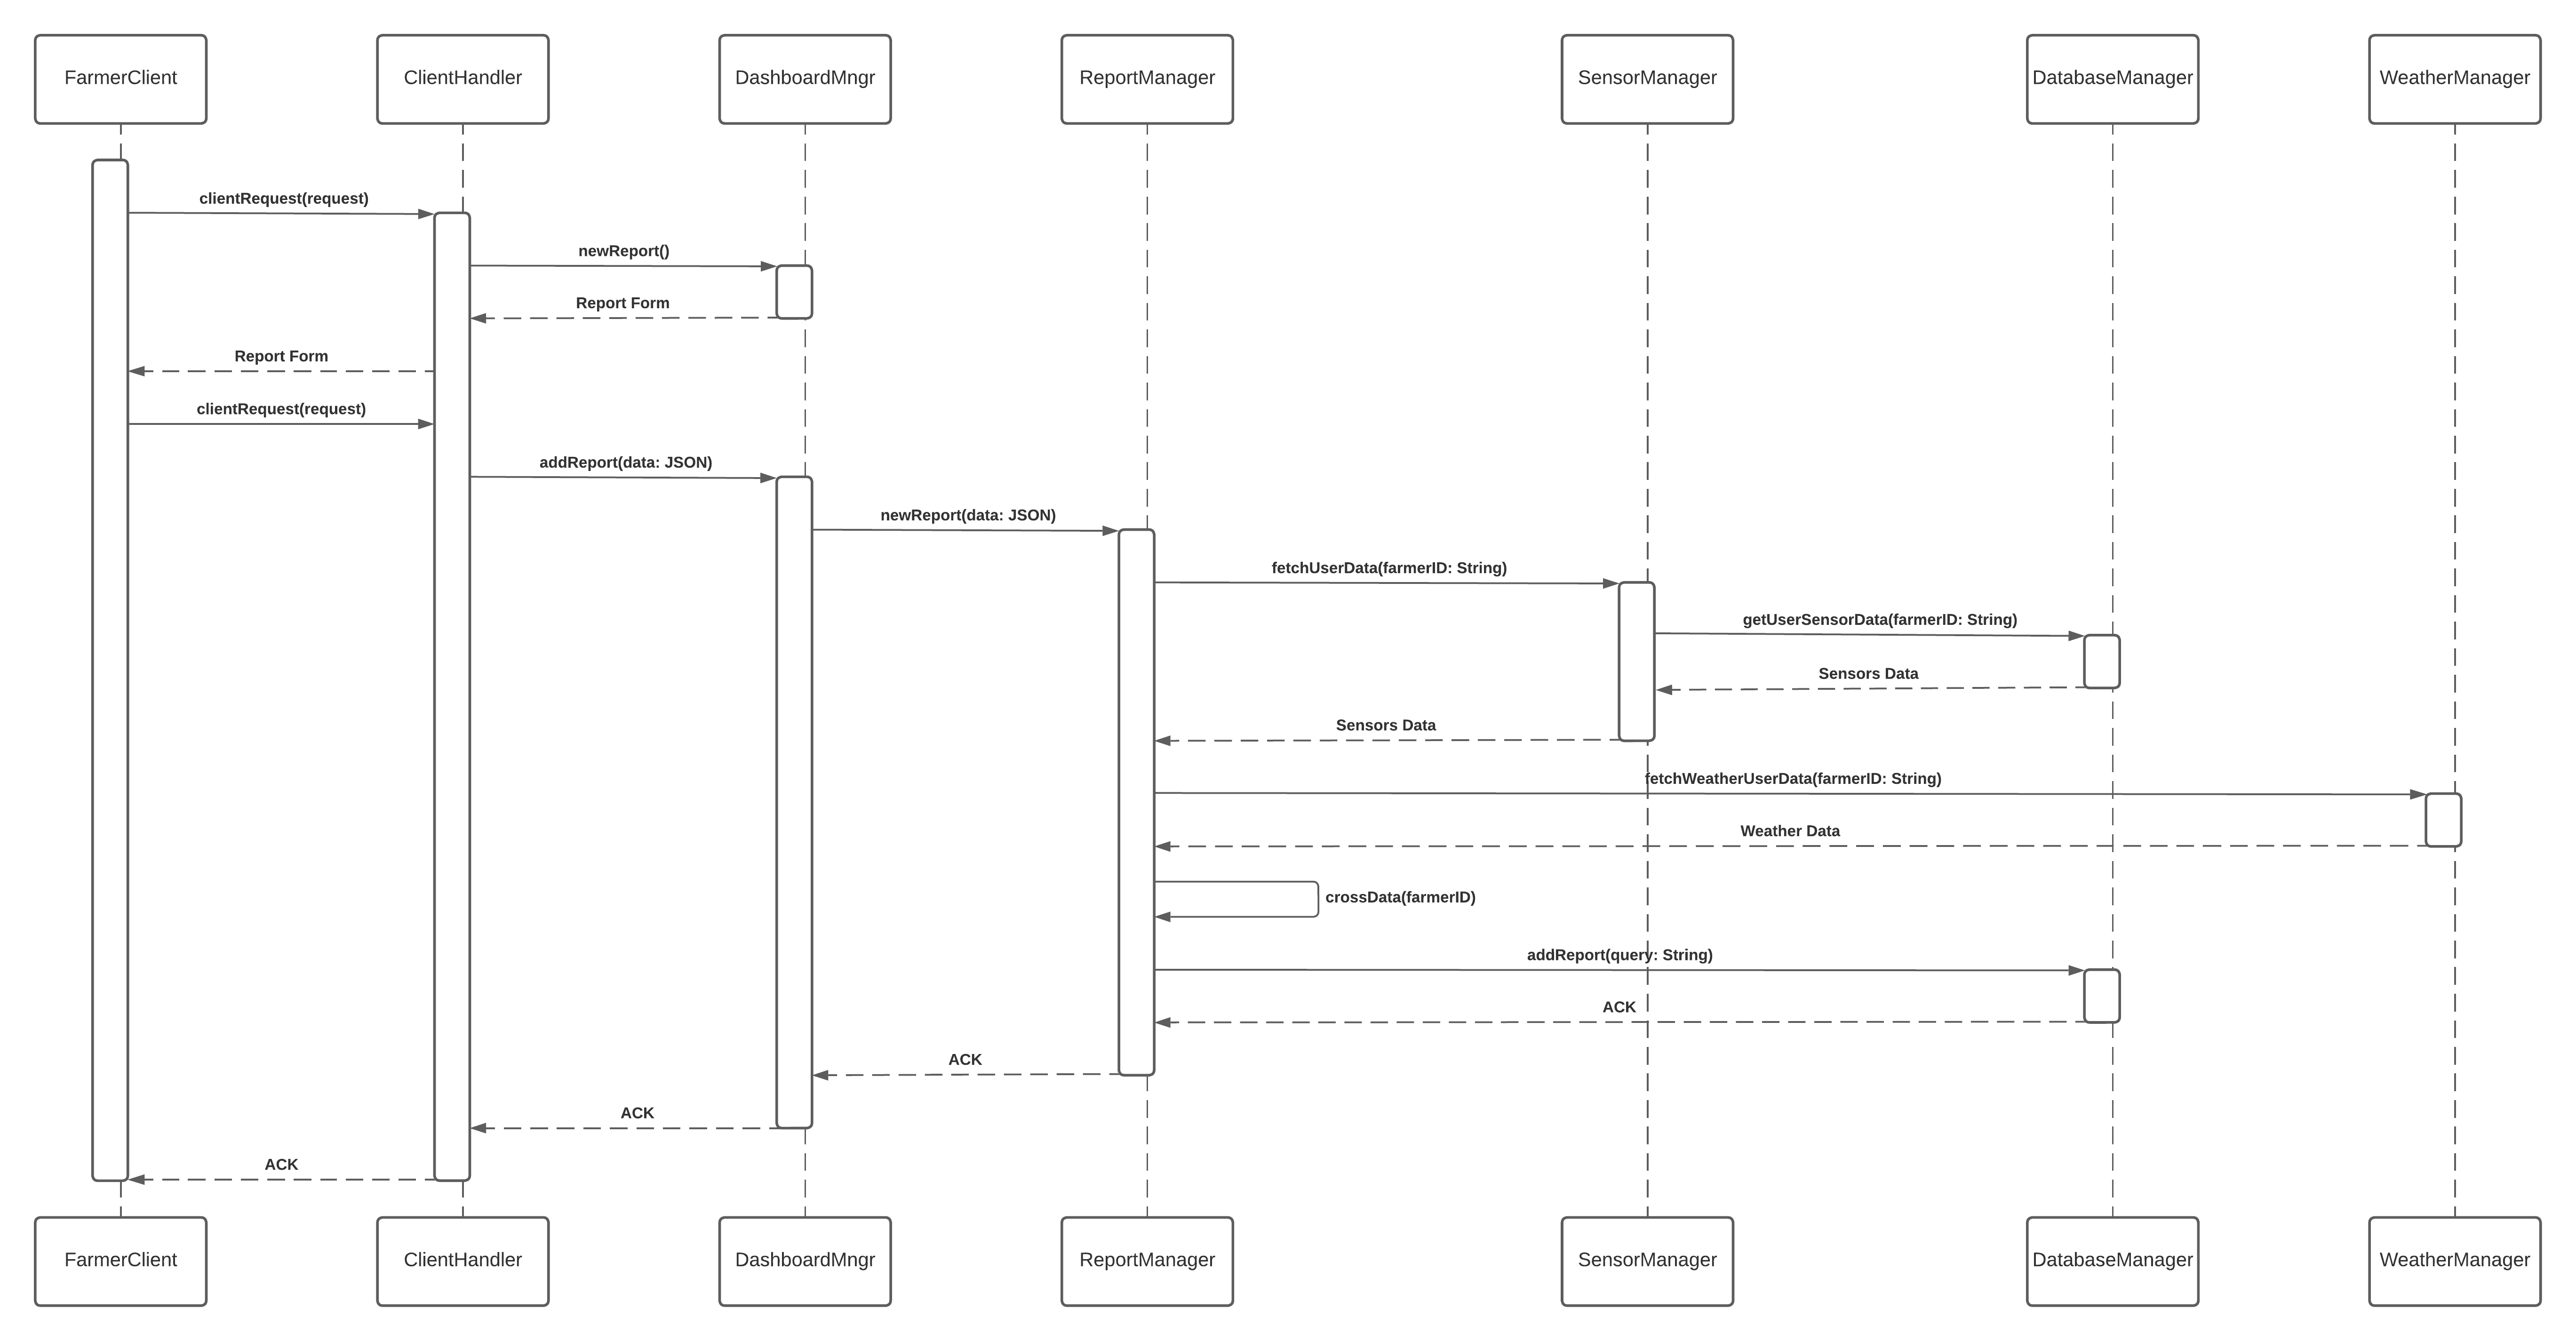
\includegraphics[scale=0.25]{images/rv/insertReport.png}
    \caption{Report insertion runtime diagram}
    \label{fig:r_report}
\end{figure}
\subsubsection{Creation and handling of a help request}
In Figure \ref{fig:r_hr1} and Figure \ref{fig:r_hr2} is described the process of creation and handling of a help request.\\
Figure \ref{fig:r_hr1} describes the creation process, which starts with a request from the farmer to get the report creation form webpage, provided by the Dashboard Manager.
Once the form is compiled, the help request is submitted and handled by the Help Request Manager, which stores it into the database. The user is then acknowledged of the success
of the operation.\\
\begin{figure}[h]
    \centering
    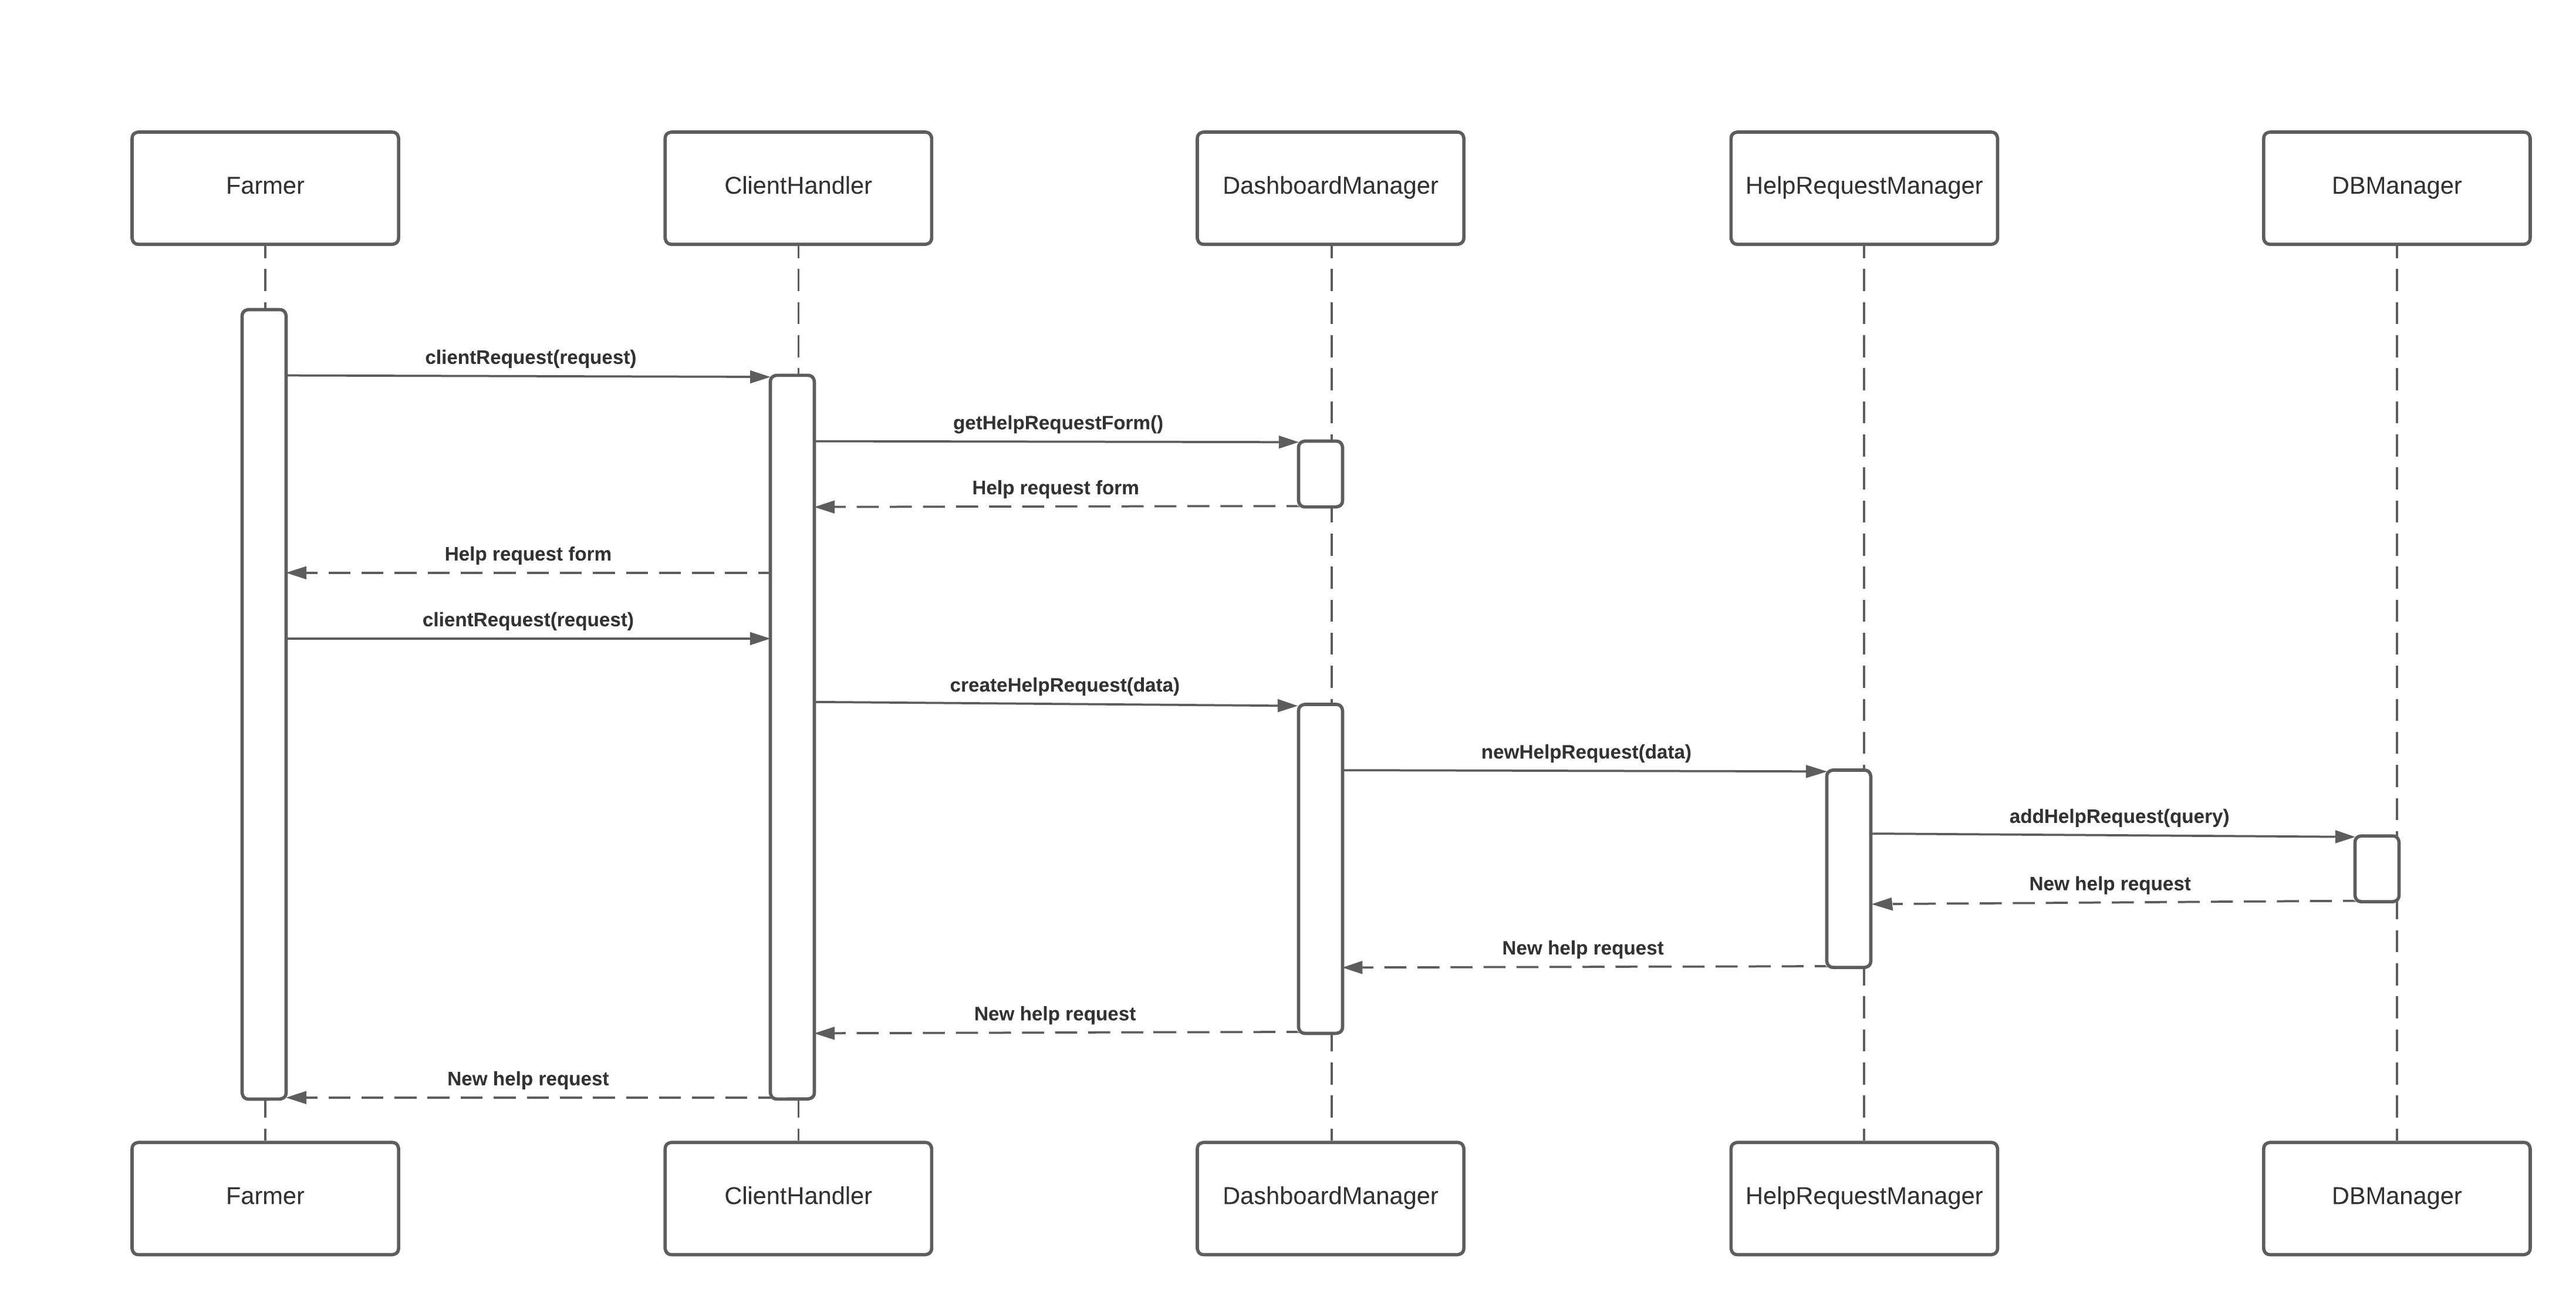
\includegraphics[scale=0.3]{images/rv/helpRequestCreation.png}
    \caption{Help request creation runtime diagram}
    \label{fig:r_hr1}
\end{figure}
Figure \ref{fig:r_hr2} describes the handling of a newly created help request by the policy makers. This process starts by getting the list of help requests, provided as a webpage
by the Dashboard Manager after fetching help requests from the database through the Help Request Manager.
Once a help request is selected, the first operation is to open it. After that, the policy maker proceeds to evaluate its severity. If the severity is low, the Help Request Manager
fetches from the database suggestions related to the help request farmer, and these suggestions are automatically sent to the farmer via e-mail by the Mail Manager.
If the severity is high, control visits to the farmer are newly scheduled and the farmer is notified via e-mail.\\
The process ends with an evaluation of the farmer performances: if they are improved the help request is closed, otherwise its severity is increased and new actions are taken.
\begin{figure}[h]
    \centering
    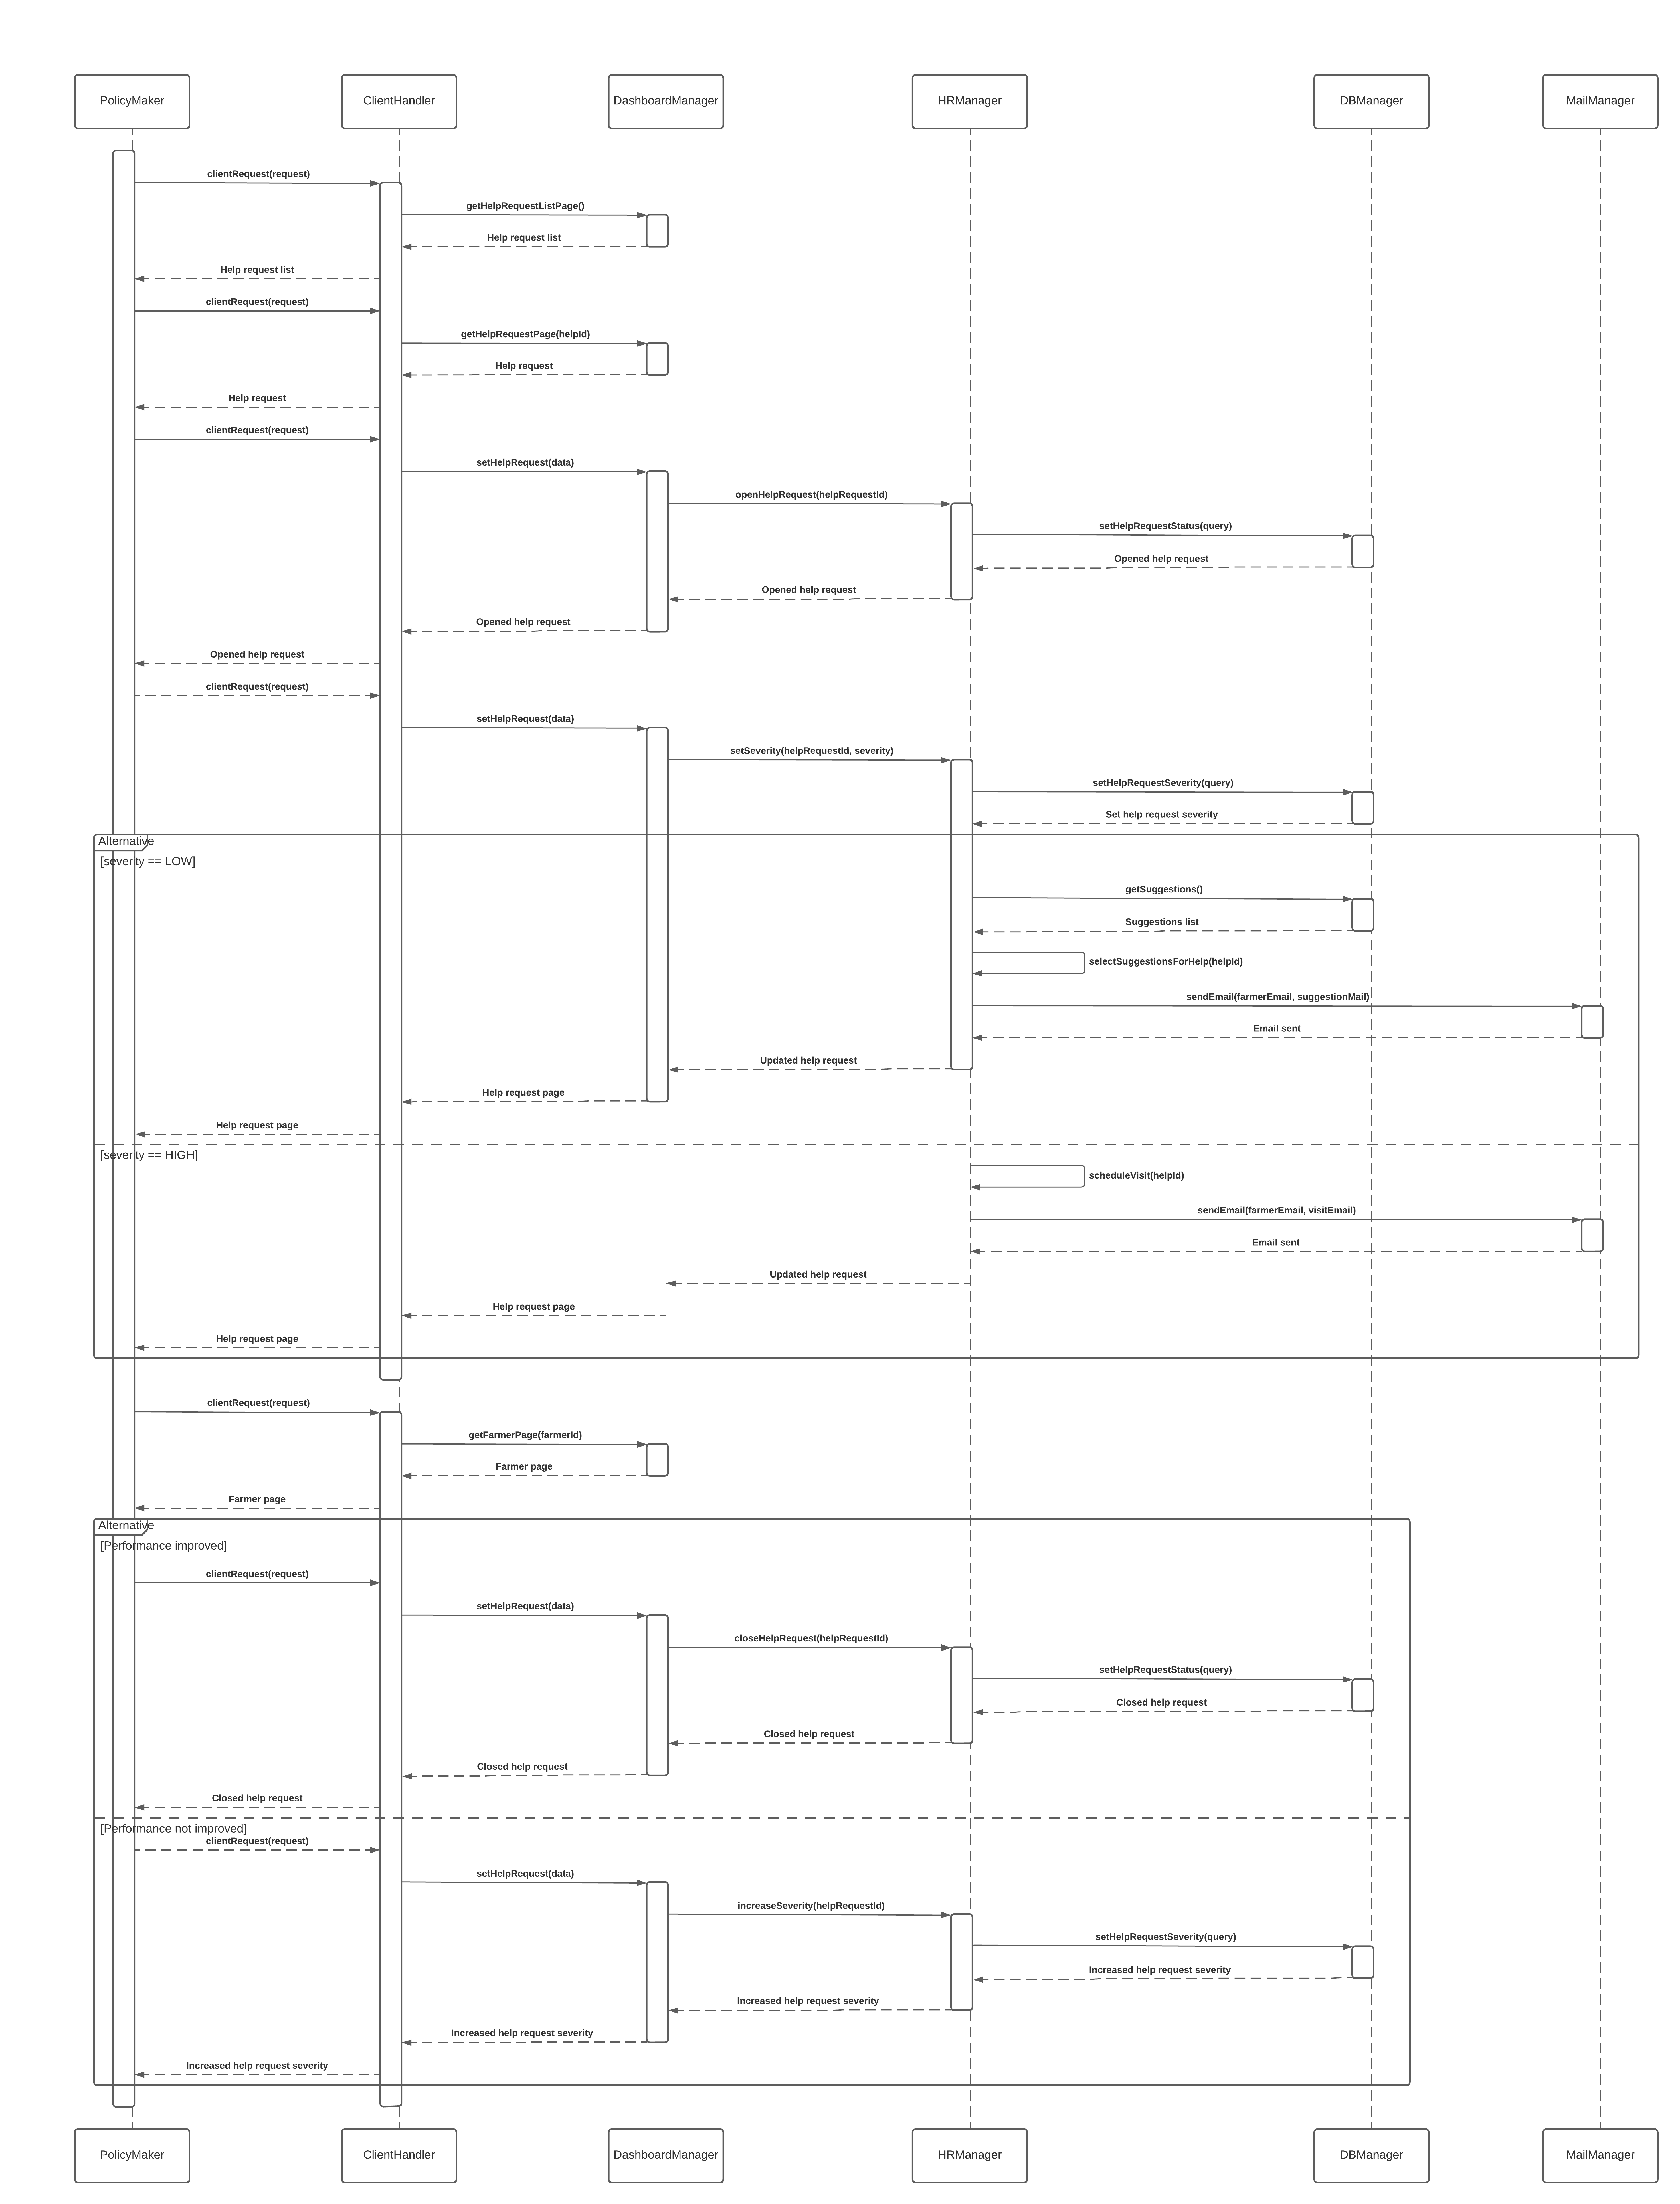
\includegraphics[scale=0.22]{images/rv/helpRequestHandling.png}
    \caption{Help request handling runtime diagram}
    \label{fig:r_hr2}
\end{figure}
\subsubsection{Forum interaction}
Figure \ref{fig:r_forum} describes a user interaction with the DREAM forum. A typical user/forum interaction would start with the opening of the forum webpage, provided by the Dashboard Manager,
where threads fetched by the Forum Manager are displayed. The next step is to open a thread discussion, which consists in a similar interaction as the previous one. If then the user intends to contribute
to the discussion by posting an answer, the user request is handled by the Forum Manager, updating the thread and storing the contribution into the database. Once the operation has succeeded, the user
is provided with the updated thread discussion webpage.
\begin{figure}[h]
    \centering
    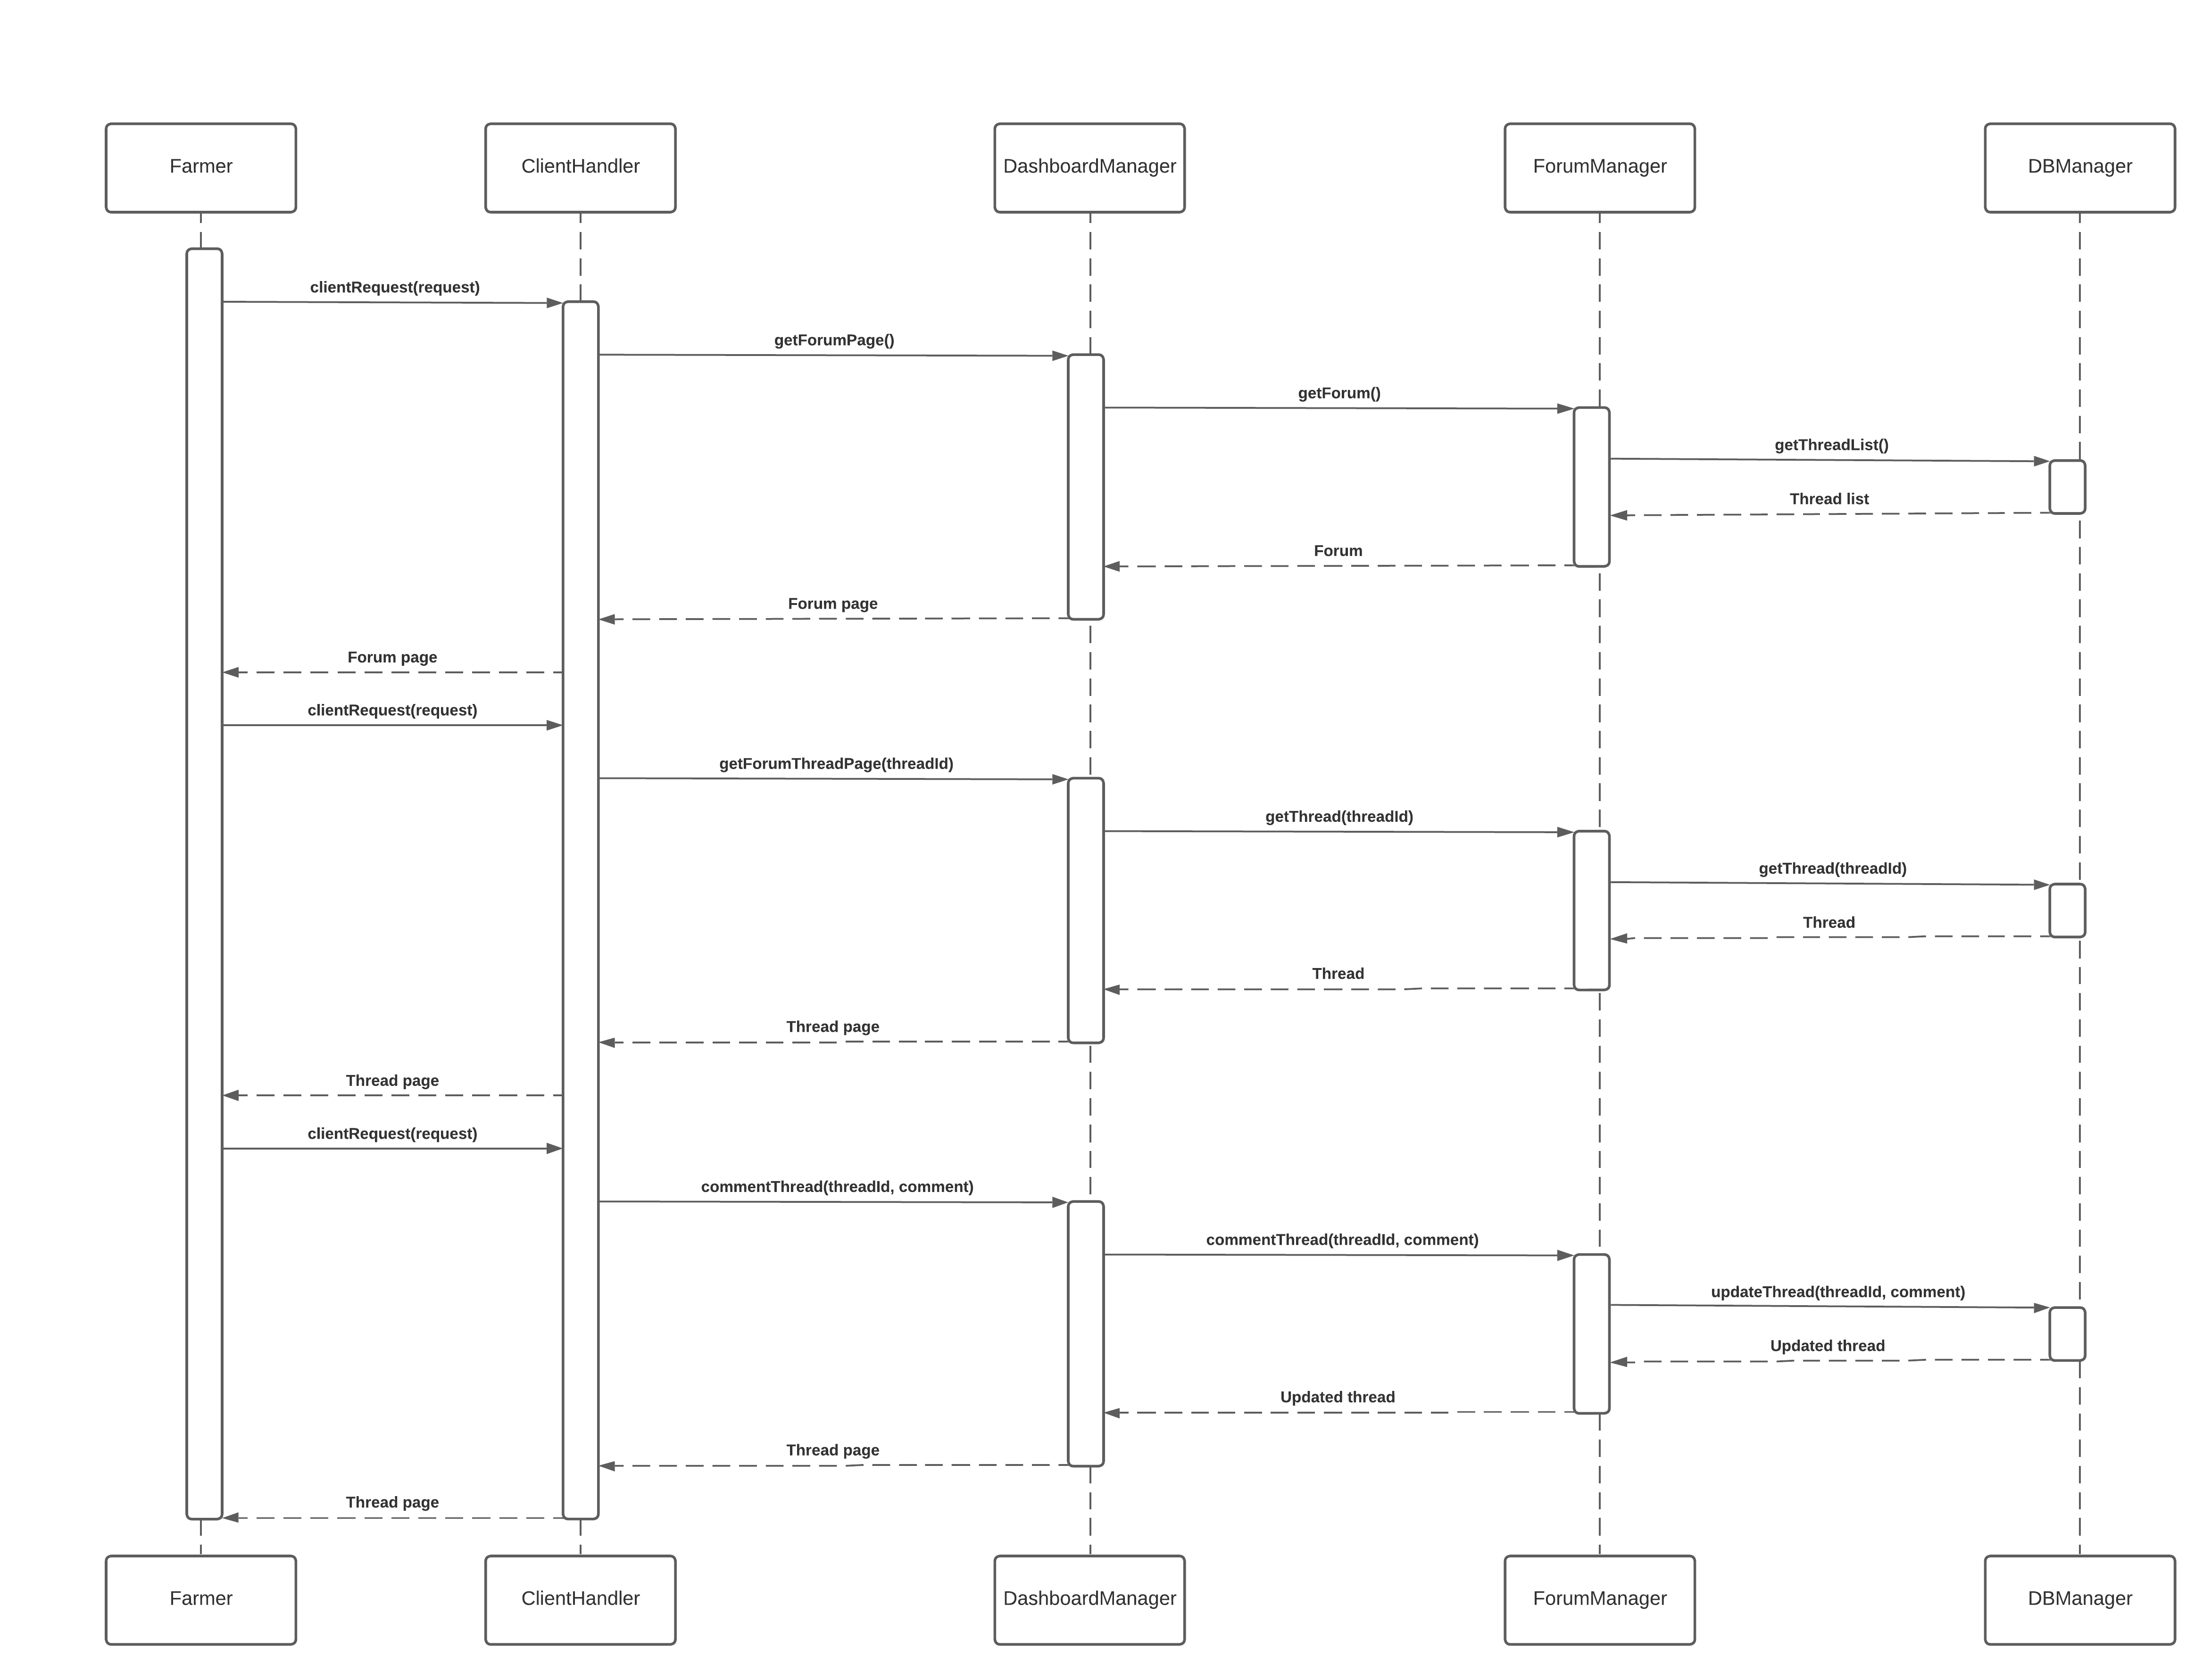
\includegraphics[scale=0.3]{images/rv/answerForum.png}
    \caption{Forum interaction runtime diagram}
    \label{fig:r_forum}
\end{figure}
\subsection{Component Interfaces}
This section lists all the methods exposed by each interface to the external components. Only internal components of the application server are described.
For each method, its parameters and its return value are only meant to give an idea of its behaviour. The list of methods may not comprehend every method
used by each interface at the end of the implementation, but should give an overall description of the main functionalities of the interfaces. Additional methods
may be added, if necessary, during the implementation phase.
\begin{itemize}
    \item \textbf{Farmer Interface}
    \begin{itemize}
        \item clientRequest(httpRequest): HttpResponse
    \end{itemize}
    \item \textbf{PM Interface}
    \begin{itemize}
        \item clientRequest(httpRequest): HttpResponse
    \end{itemize}
    \item \textbf{SH Interface}
    \begin{itemize}
        \item postSensorData(sensorData): void
    \end{itemize}
    \item \textbf{Irrigation Interface}
    \begin{itemize}
        \item postSensorData(sensorData): void
    \end{itemize}
    \item \textbf{Sensor Manager Interface}
    \begin{itemize}
        \item fetchUserData(farmerID, date): List$<$SensorData$>$
        \item storeSensorData(sensorData): void
    \end{itemize}
    \item \textbf{Access Manager Interface}
    \begin{itemize}
        \item authUser(email, password): User
        \item getAuthenticatedUser(): User
        \item addnewCredentials(data): void
    \end{itemize}
    \item \textbf{Dashboard Interface}
    \begin{itemize}
        \item getLoginPage(loginFailed): DashboardPage
        \item getHomepage(): DashboardPage
        \item buildHomepage(): DashboardPage
        \item getReportPage(): DashboardPage
        \item getReportForm(): DashboardPage
        \item addReport(data): DashboardPage
        \item getProductListPage(): DashboardPage
        \item getProductPage(): DashboardPage
        \item getForumPage(): DashboardPage
        \item getForumThreadPage(): DashboardPage
        \item createThread(data): DashboardPage
        \item commentThread(threadId, data): DashboardPage 
        \item getFarmerPage(farmerId): DashboardPage
        \item getHelpRequestListPage(): DashboardPage
        \item getHelpRequestPage(helpId): DashboardPage
        \item getHelpRequestForm(): DashboardPage
        \item getForecastPage(): DashboardPage
        \item createHelpRequest(data): DashboardPage
    \end{itemize}
    \item \textbf{User Manager Interface}
    \begin{itemize}
        \item getUser(userId): User
        \item getUserList(limit): List$<$User$>$ 
        \item fetchFarmerPerformance(farmerID)
    \end{itemize}
    \item \textbf{Forum Interface}
    \begin{itemize}
        \item getForum(): Forum
        \item getThread(threadId): Thread 
        \item commentThread(threadId, comment): Thread
    \end{itemize}
    \item \textbf{HR Interface}
    \begin{itemize}
        \item newHelpRequest(data): HelpRequest
        \item fetchHelpRequests(): List$<$HelpRequest$>$
        \item forwardVisitScheduling(farmerID, visitData): Date
        \item forwardSuggestion(farmerID, suggestion)
        \item closeHelpRequest(requestID)
        \item openHelpRequest(requestId): HelpRequest
        \item closeHelpRequest(requestID): HelpRequest
        \item setSeverity(requestID, severity): HelpRequest
        \item increaseSeverity(requestID): HelpRequest
    \end{itemize}
    \item \textbf{Report Interface}
    \begin{itemize}
        \item newReport(data): Report
        \item crossData(farmerId): Report
    \end{itemize}
    \item \textbf{Weather Interface}
    \begin{itemize}
        \item fetchWeatherData(locationId): WeatherData
    \end{itemize}
    \item \textbf{Mail Manager Interface}
    \begin{itemize}
        \item sendEmail(emailAddress, mailData): JSONObject
    \end{itemize}
    \item \textbf{DBM Interface}
    \begin{itemize}
        \item addCredentials(String query): void
        \item checkCredentials(email, password): boolean
        \item addReport(query): Report
        \item getUserSensorData(farmerID): List$<$SensorData$>$
        \item saveIrrigationData(query): SensorData
        \item getFarmerPerformance(query): List$<$FarmerPerformance$>$
        \item getHelpRequests(): List$<$HelpRequest$>$
        \item addHelpRequest(query): HelpRequest
        \item setHelpRequestStatus(query): HelpRequest
        \item setHelpRequestSeverity(query): HelpRequest
        \item getThreadList(): List$<$Thread$>$
        \item getThread(threadId): Thread
        \item updateThread(threadId, comment): Thread
    \end{itemize}
\end{itemize}
\subsection{Selected Architectural styles and patterns}
\begin{itemize}
    \item \textbf{Three-Tier Architecture}\\A three-tier architecture was chosen for the 
    implementation of the DREAM platform: presentation, application, and data tier. 
    The key three-tier benefit is improved scalability, since each element
    can scale horizontally and the application servers can be deployed on many machines. 
    Also, the database does not make connections with every client, it only requires 
    connections from a smaller number of application servers. This architecture also leads to 
    implement thin clients. \\
    Change management is easier and faster to execute, because program logic
     is implemented on the centralized server, so the modularity makes it easier to modify 
     or replace one tier without affecting the other tier.
    \item \textbf{REST API}\\It was decided to implement the interfaces intended for web services 
    following the standards imposed by the REST architectural style. This choice was made for ease 
    of development and increased scalability of the system, in fact, thanks to the flexibility of 
    RESTful APIs, it will be possible to add components to the system or modify them easily.  
    \item \textbf{Model-View-Controller}\\
    The application software is implemented following the MVC design pattern, splitting the application logic into presentation logic (view),
    business logic (controller) and data management logic (model). This pattern follows the deployment architecture and allows an easy defining
    of each component's tasks. In detail, the design pattern implemented in the DREAM application does not follow the standard MVC, where there is also 
    interaction between the View and the Model, but the Cocoa MVC pattern where this kind of interaction does not exist and each communication between View and Model
    is first processed by the Controller layer.
    \begin{figure}[h]
        \centering
        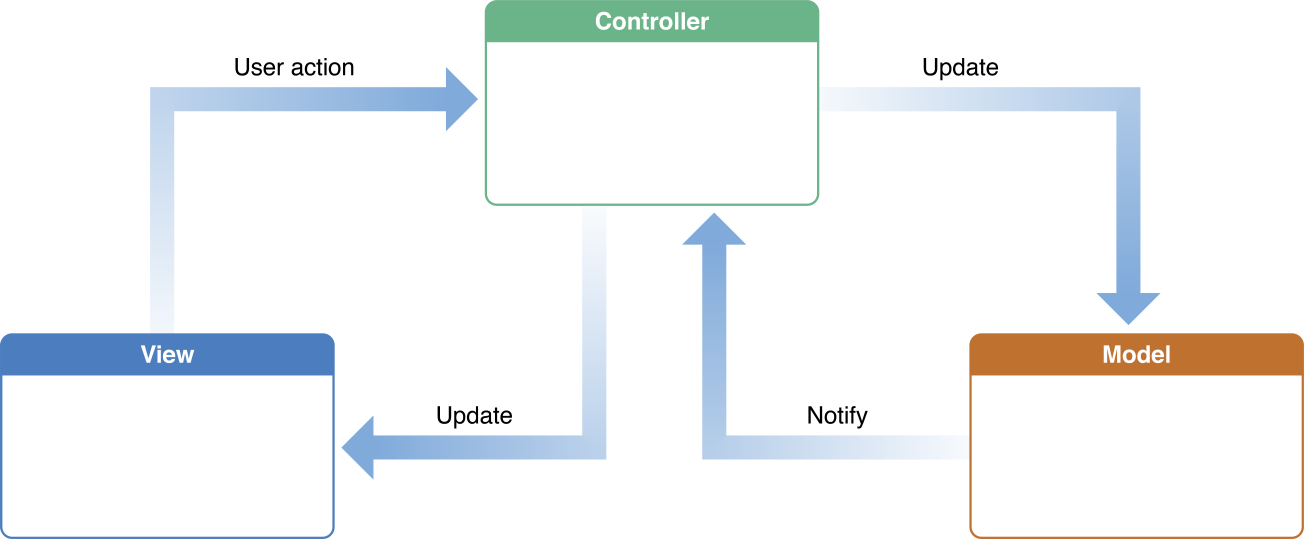
\includegraphics[scale=0.23]{images/cocoamvc.png}
        \caption{Cocoa Model-View-Controller}
        \label{fig:mvc}
    \end{figure}
    \item \textbf{Event based communication for sensors}\\The communication protocol chosen to retrieve 
    data created by IoT sensors is Message Queue Telemetry Transport (MQTT), a standard messaging 
    protocol for the Internet of Things that is extremely lightweight and ideal for connecting remote 
    devices with a small code footprint and minimal network bandwidth. MQTT is a publish/subscribe 
    communication protocol: A topic will be created for each farmer, then the sensors, depending on 
    their geographical location, will publish data to the topics corresponding to the farmers of 
    their interest. In this way it will be possible to access the data created by the sensors divided 
    by each farmer. A MQTT Broker Cluster distributed in the region of Telangana, will take care of 
    the management of sensor data. The application server will be subscribed to all topics and will 
    receive periodically the data, it will then store them in the database to make them always 
    accessible for processing.
    This design provides high scalability because, if we had to resort to replication of the 
    application server, it will be enough to subscribe to all topics the new server to receive 
    all sensor data.
    \begin{figure}[h]
        \centering
        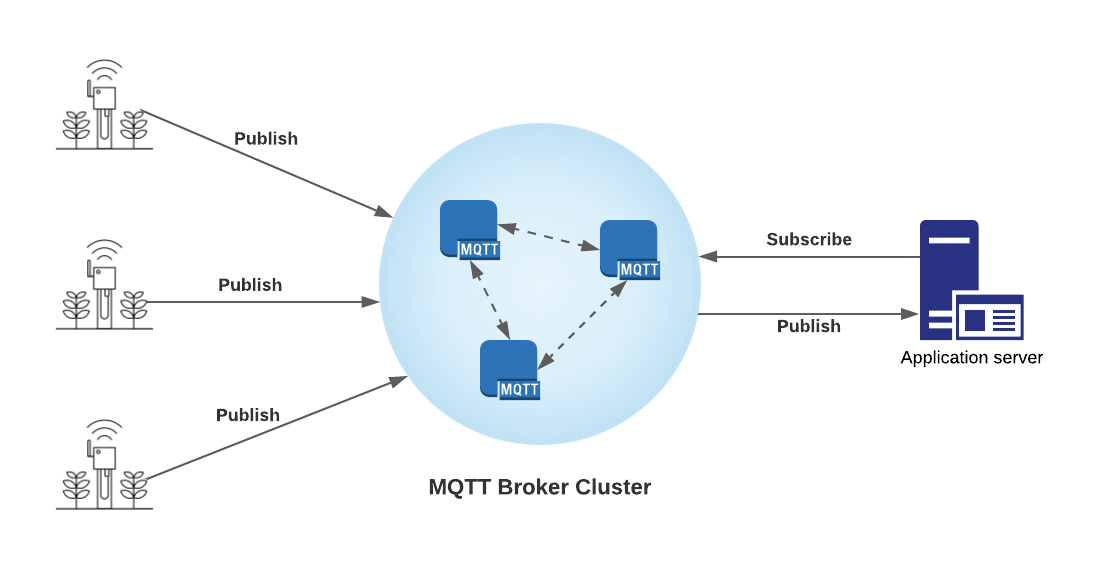
\includegraphics[scale=0.68]{images/mqtt.png}
        \caption{Distributed MQTT Broker System}
        \label{fig:mqtt}
    \end{figure}
\end{itemize}
\subsection{Other design decisions}
\begin{itemize}
    \item \textbf{Thin Clients}\\The architecture has been designed so that the end-points of the system 
    are thin clients, i.e. they use resources hosted within a central server, which therefore do not need an high 
    computational power. A thin client connects to a server-based environment that hosts the majority of 
    applications, memory, and sensitive data the user needs. It was decided to undertake this solution 
    to ensure that farmers who do not have powerful devices can use the platform without complications.
\end{itemize}
\section{User Interface Desgin} %l'impaginazione la facciamo alla fine
The following section describes the user interface of the DREAM webapp. Its goal is to motivate design choices, 
describe each mockup, its content and the flow between the various pages of the application.
The section is divided in three subsections: the first one focuses on the farmer's webapp, the second one on the Policy Maker's webapp
and the third on the flow of the webapp.\\
\begin{figure}[h]
    \centering
    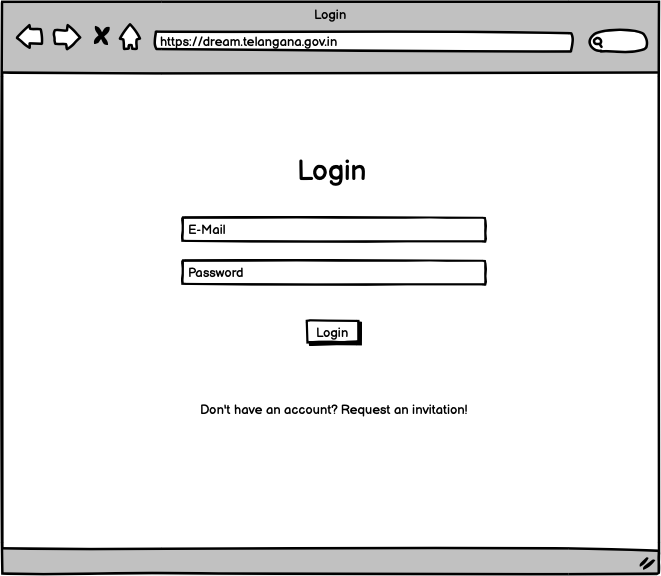
\includegraphics[scale=0.4]{images/uimockups/login.png}
    \caption{Login page}
    \label{fig:ui_login}
\end{figure}
The first page for both farmers and policy makers will always be the login page, requiring e-mail and password to login into the platform.
For farmers, this page will be accessible from any web browser and will also show an option to request an invitation: a simple popup will open up requesting
the user to insert his e-mail address, which will be then submitted to the policy makers who will handle the registration request and procedure.

\subsection{Farmers User Interface}
\begin{figure}[h]
    \centering
    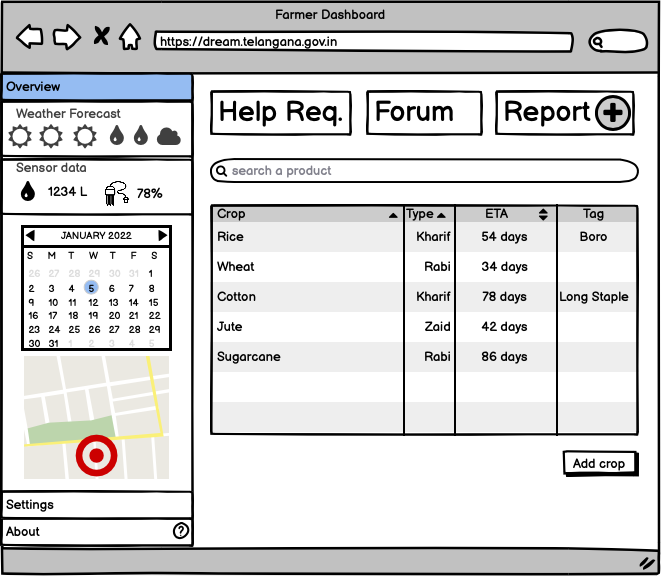
\includegraphics[scale=0.4]{images/uimockups/f_homepage.png}
    \caption{Farmer homepage}
    \label{fig:ui_f_homepage}
\end{figure}
The first page visualized by the farmer once logged in the platform is the homepage. The farmer's homepage contains a brief overview of weather forecasts
and sensor data, and allows users to keep track of their crop in a table containing information about crop's type, eta and comments. The user can add crops 
to the table by clicking "Add crop", which will open a popup to insert the new crop and its info. The page then allows to navigate to the pages for creating reports
and help request, to the forum or to a specific product page by searching the product by its name.\\
\begin{figure}[h]
    \centering
    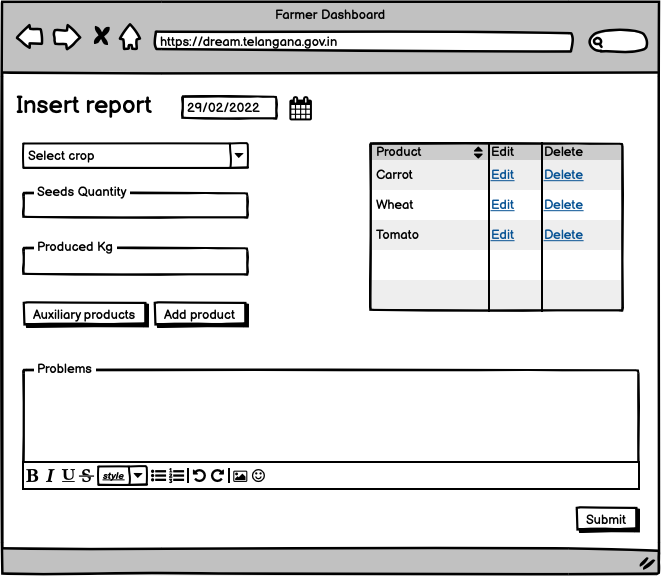
\includegraphics[scale=0.4]{images/uimockups/f_report.png}
    \caption{Farmer's report creation page}
    \label{fig:ui_f_report}
\end{figure}
The report creation page consists of a simple form to insert the harvested products and their quantity. Each product added to the report is visualized 
on a table, that also allows to edit or delete previously added products. To add a product, the user selects the type of product by an interactive dropdown
menu that also allows searching the product, then adds seeds and produced quantity. Clicking on "Auxiliary Products" will open a popup showing the auxiliary
products used in the harvesting process, allowing the user to add, edit or remove them. Once the user has inserted all the necessary information, by clicking on "Add product"
the product will be added to the report's products. The page also contains a text area where the user can insert the problems encountered during the harvesting process. 
Once the report is fully compiled, clicking on "Submit" will create the report and send it to the DREAM server. The webapp will then rediredt the user to the homepage. \\
\begin{figure}[h]
    \centering
    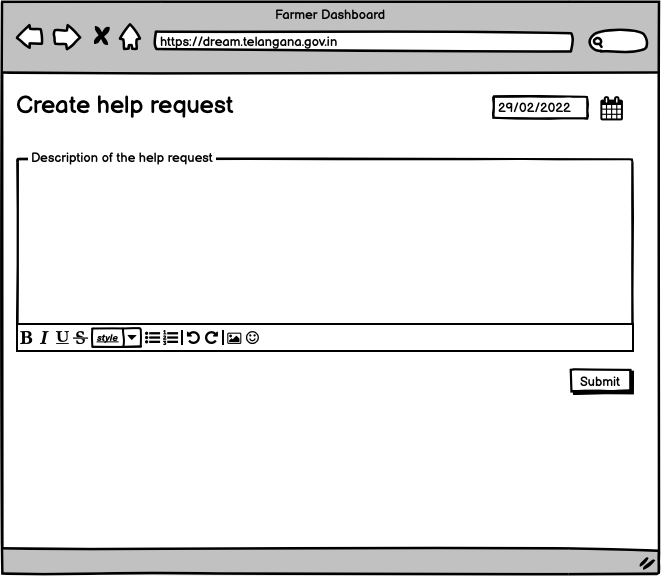
\includegraphics[scale=0.4]{images/uimockups/f_helprequest.png}
    \caption{Farmer's help request creation page}
    \label{fig:ui_f_helprequest}
\end{figure}
\begin{figure}[h]
    \centering
    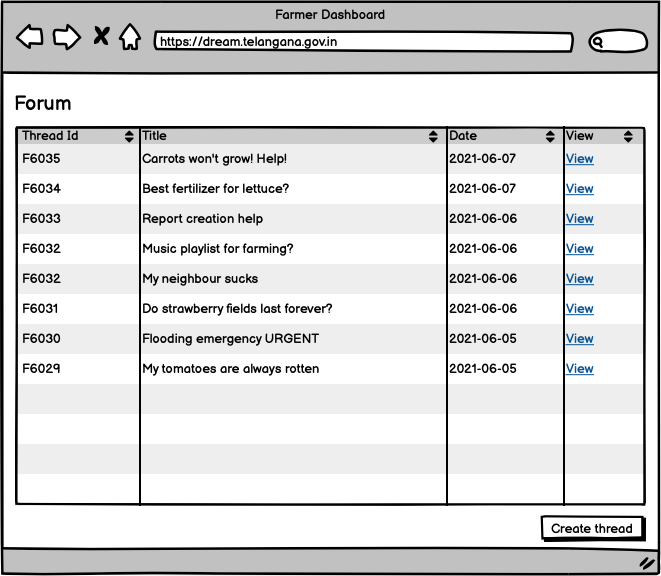
\includegraphics[scale=0.4]{images/uimockups/f_forum.png}
    \caption{Farmer's forum page}
    \label{fig:ui_f_forum}
\end{figure}
The forum page shows all the open threads, allowing the user to open them and visualize the discussion.
A farmer can also create a new thread by clicking "Create thread", which will redirect the user to the thread creation page.\\
\begin{figure}[h]
    \centering
    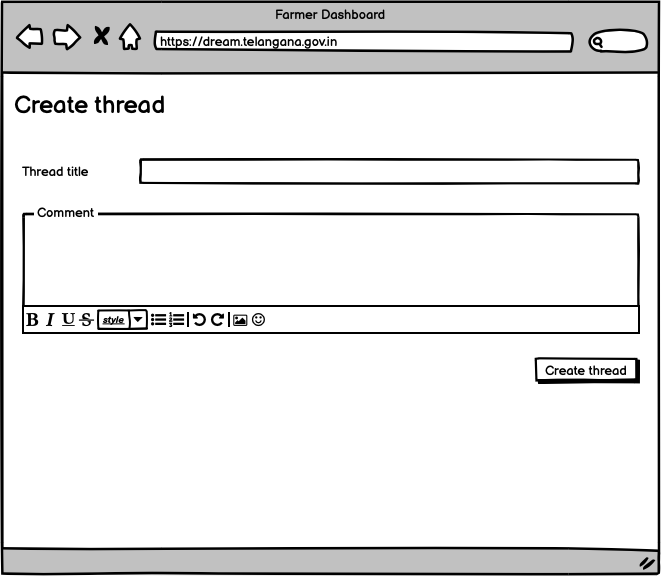
\includegraphics[scale=0.4]{images/uimockups/f_forumcreatethread.png}
    \caption{Farmer's thread creation page}
    \label{fig:ui_f_forumcreatethread}
\end{figure}
\begin{figure}[h]
    \centering
    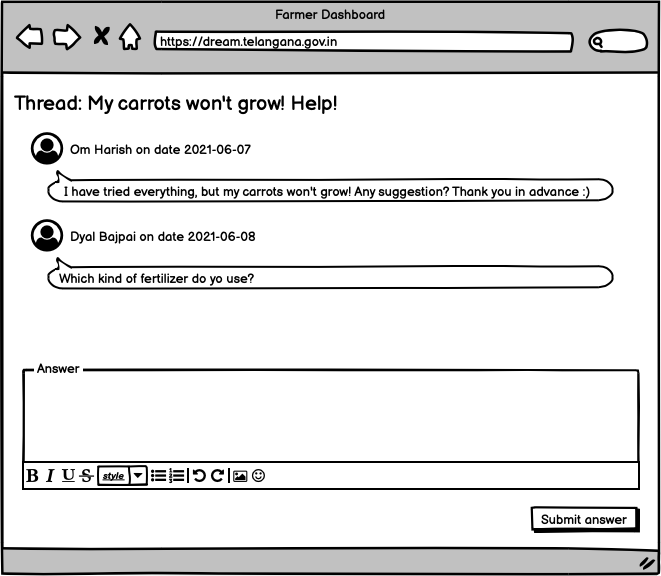
\includegraphics[scale=0.4]{images/uimockups/f_forumthread.png}
    \caption{Farmer's thread page}
    \label{fig:ui_f_forumthread}
\end{figure}
\begin{figure}[h]
    \centering
    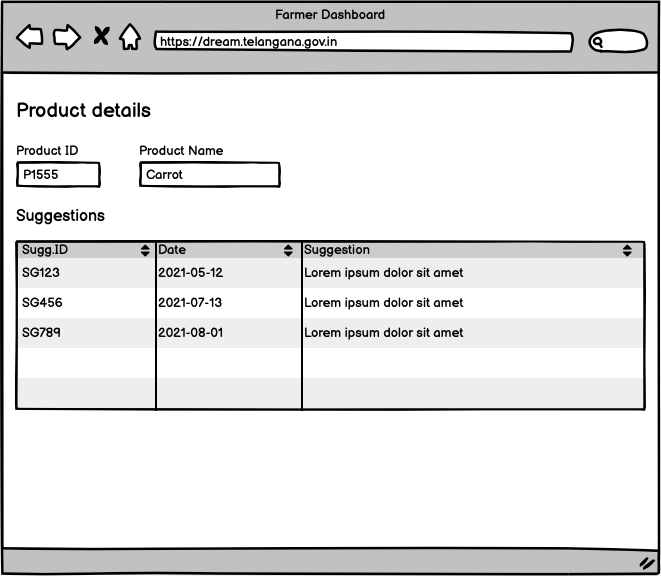
\includegraphics[scale=0.4]{images/uimockups/f_product.png}
    \caption{Farmer's product page}
    \label{fig:ui_f_product}
\end{figure}

\subsection{Policy maker User Interface}
\begin{figure}[h]
    \centering
    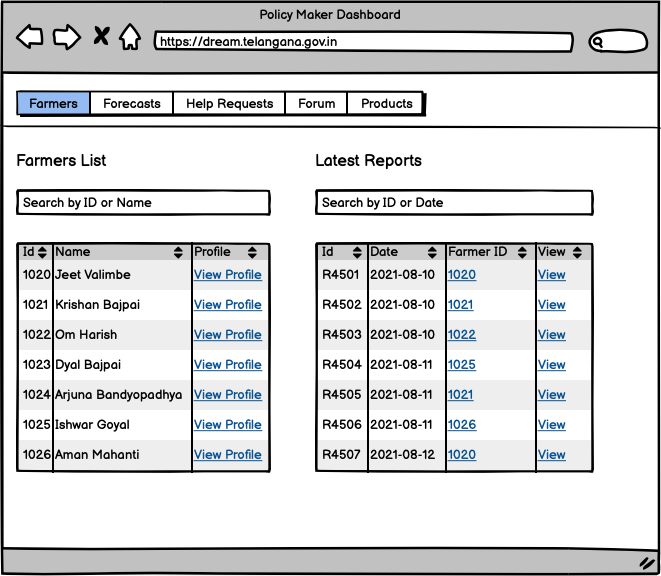
\includegraphics[scale=0.4]{images/uimockups/pm_farmers.png}
    \caption{Policy maker's farmers page}
    \label{fig:ui_pm_farmers}
\end{figure}
The first page visualized by the policy maker once logged into the platform lists the farmers and the latest reports submitted, allowing the
user to search farmers/reports. The user can then navigate to the farmer/report details. On the top of the page there is a navigation bar that
allows the user to switch dashboard page.\\
\begin{figure}[h]
    \centering
    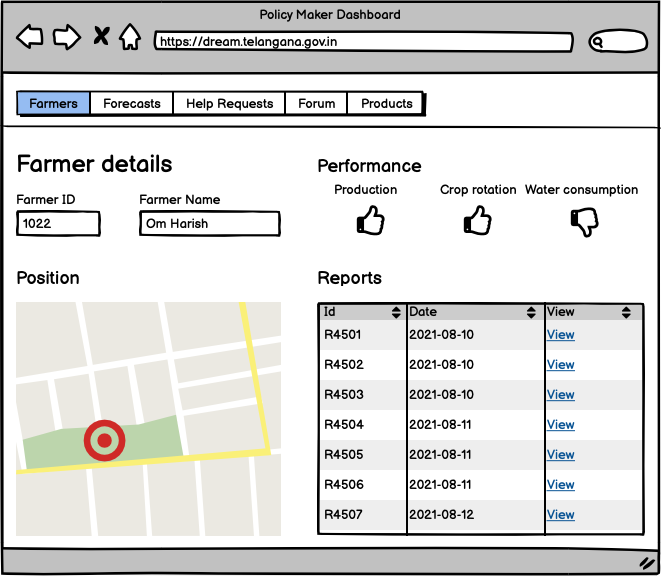
\includegraphics[scale=0.4]{images/uimockups/pm_farmerdetails.png}
    \caption{Policy maker's farmer detail page}
    \label{fig:ui_pm_farmerdetails}
\end{figure}
\begin{figure}[h]
    \centering
    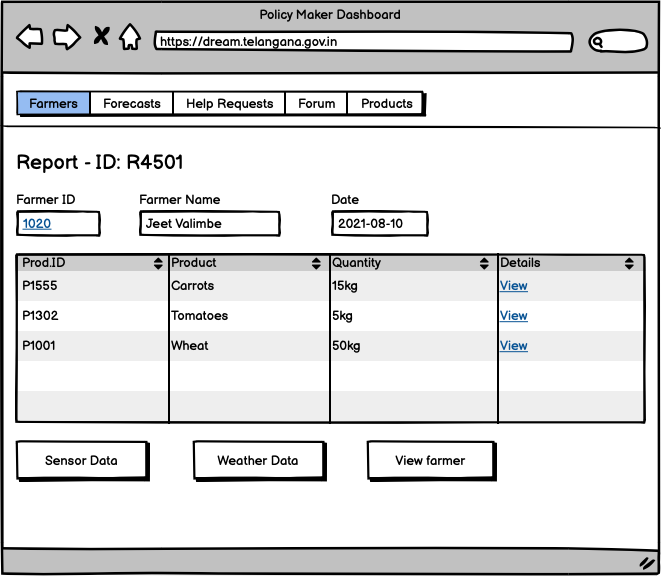
\includegraphics[scale=0.4]{images/uimockups/pm_reports.png}
    \caption{Policy maker's report page}
    \label{fig:ui_pm_reports}
\end{figure}
\begin{figure}[h]
    \centering
    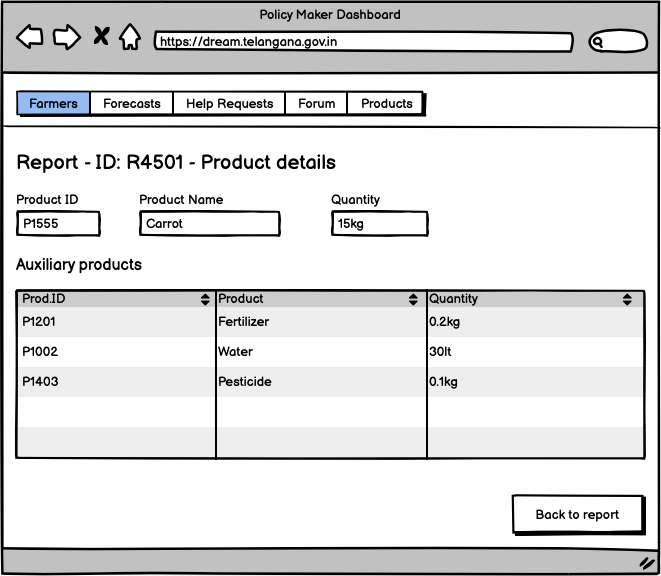
\includegraphics[scale=0.4]{images/uimockups/pm_reportproductdetail.png}
    \caption{Policy maker's report production detail page}
    \label{fig:ui_pm_reportproductdetail}
\end{figure}
\begin{figure}[h]
    \centering
    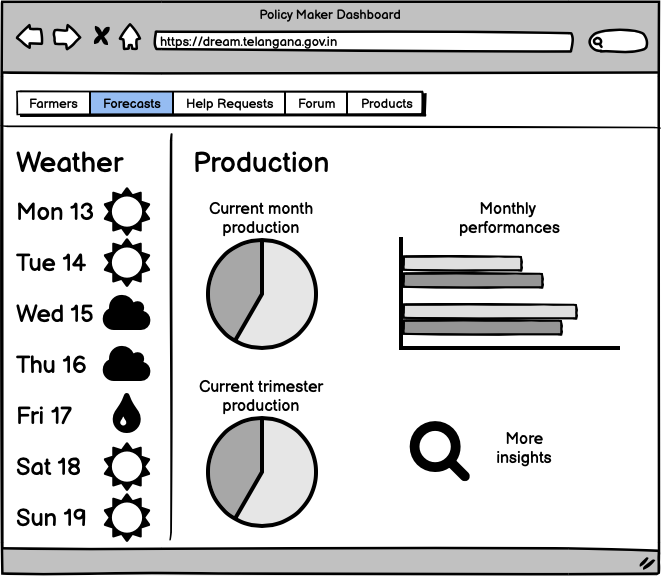
\includegraphics[scale=0.4]{images/uimockups/pm_forecasts.png}
    \caption{Policy maker's forecasts page}
    \label{fig:ui_pm_forecasts}
\end{figure}
The forecast page contains basic information about the future weather forecasts. Production forecasts are calculated and then shown to the user through
graphs.\\
\begin{figure}[h]
    \centering
    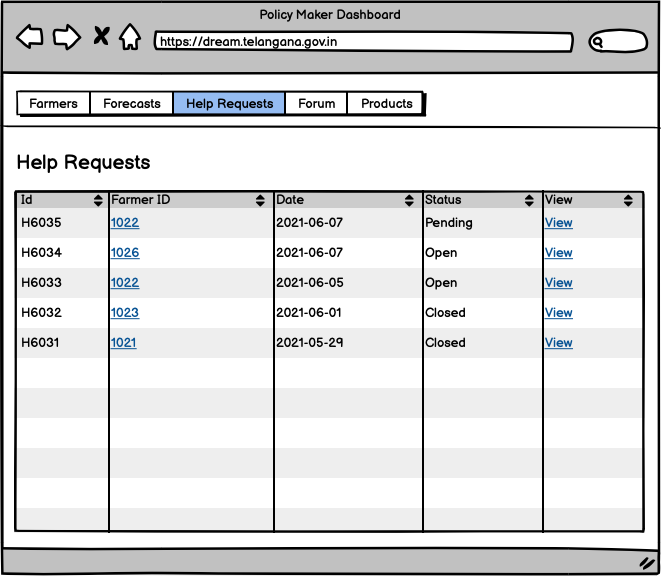
\includegraphics[scale=0.4]{images/uimockups/pm_helprequests.png}
    \caption{Policy maker's help requests page}
    \label{fig:ui_pm_helprequests}
\end{figure}
\begin{figure}[h]
    \centering
    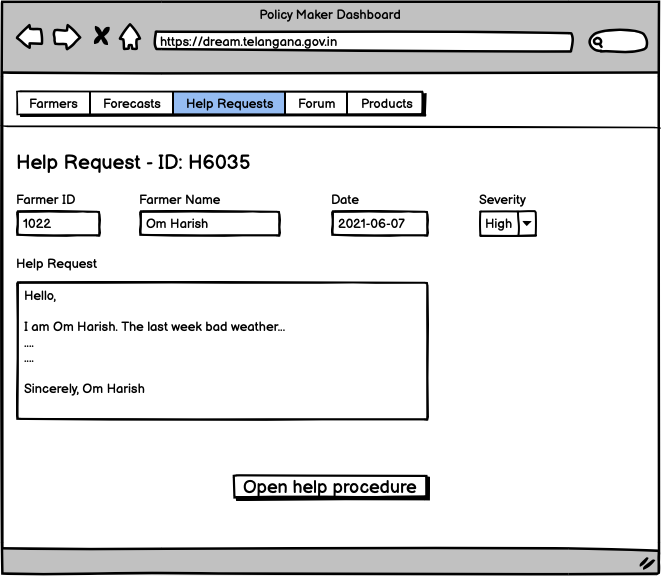
\includegraphics[scale=0.4]{images/uimockups/pm_helprequestdetail.png}
    \caption{Policy maker's help request detail page}
    \label{fig:ui_pm_helprequestdetail}
\end{figure}
\begin{figure}[h]
    \centering
    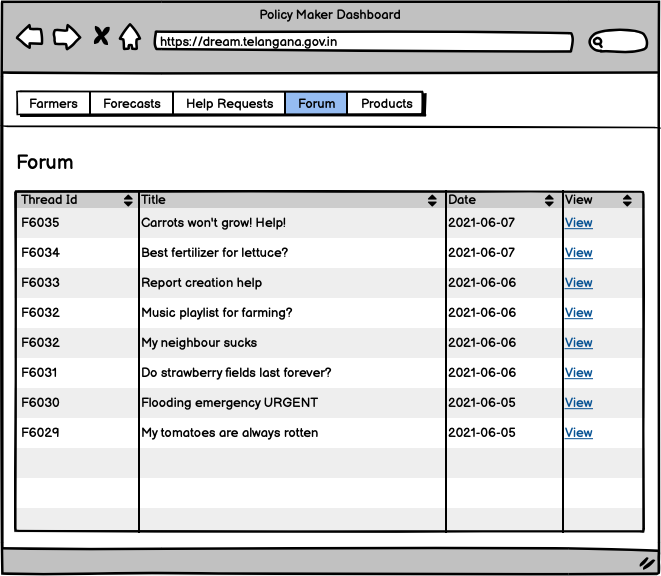
\includegraphics[scale=0.4]{images/uimockups/pm_forum.png}
    \caption{Policy maker's forum page}
    \label{fig:ui_pm_forum}
\end{figure}
\begin{figure}[h]
    \centering
    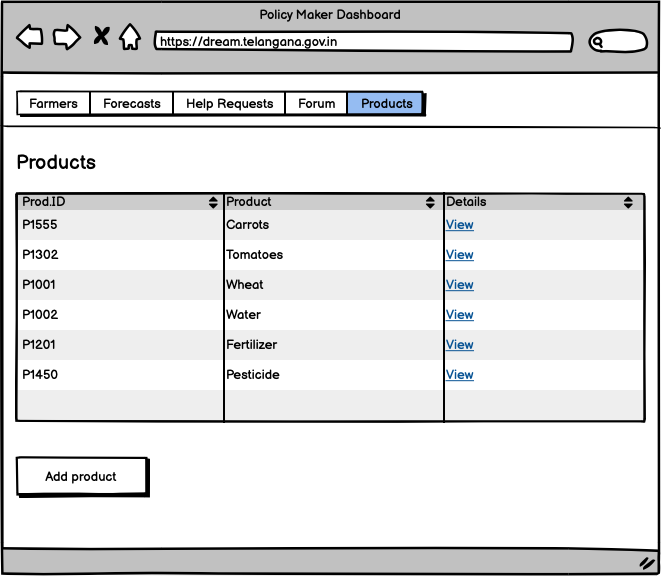
\includegraphics[scale=0.4]{images/uimockups/pm_products.png}
    \caption{Policy maker's products page}
    \label{fig:ui_pm_products}
\end{figure}
\begin{figure}[h]
    \centering
    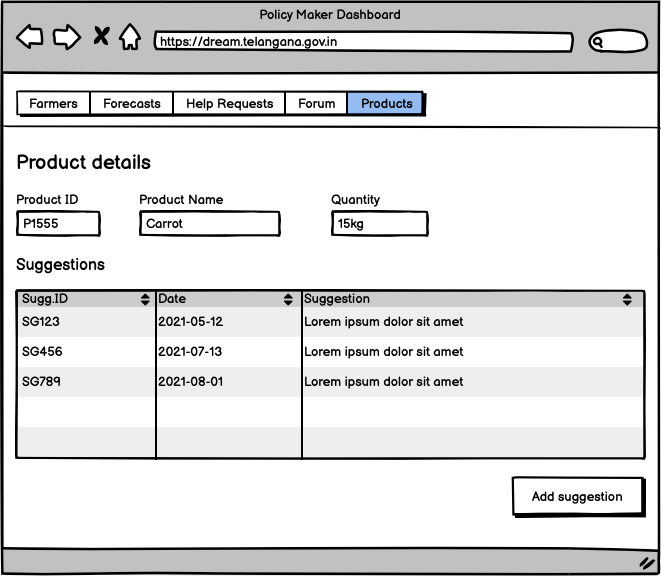
\includegraphics[scale=0.4]{images/uimockups/pm_productdetail.png}
    \caption{Policy maker's product detail page}
    \label{fig:ui_pm_productdetail}
\end{figure}

\subsection{Flow of the User Interface}
\begin{figure}[h]
    \centering
    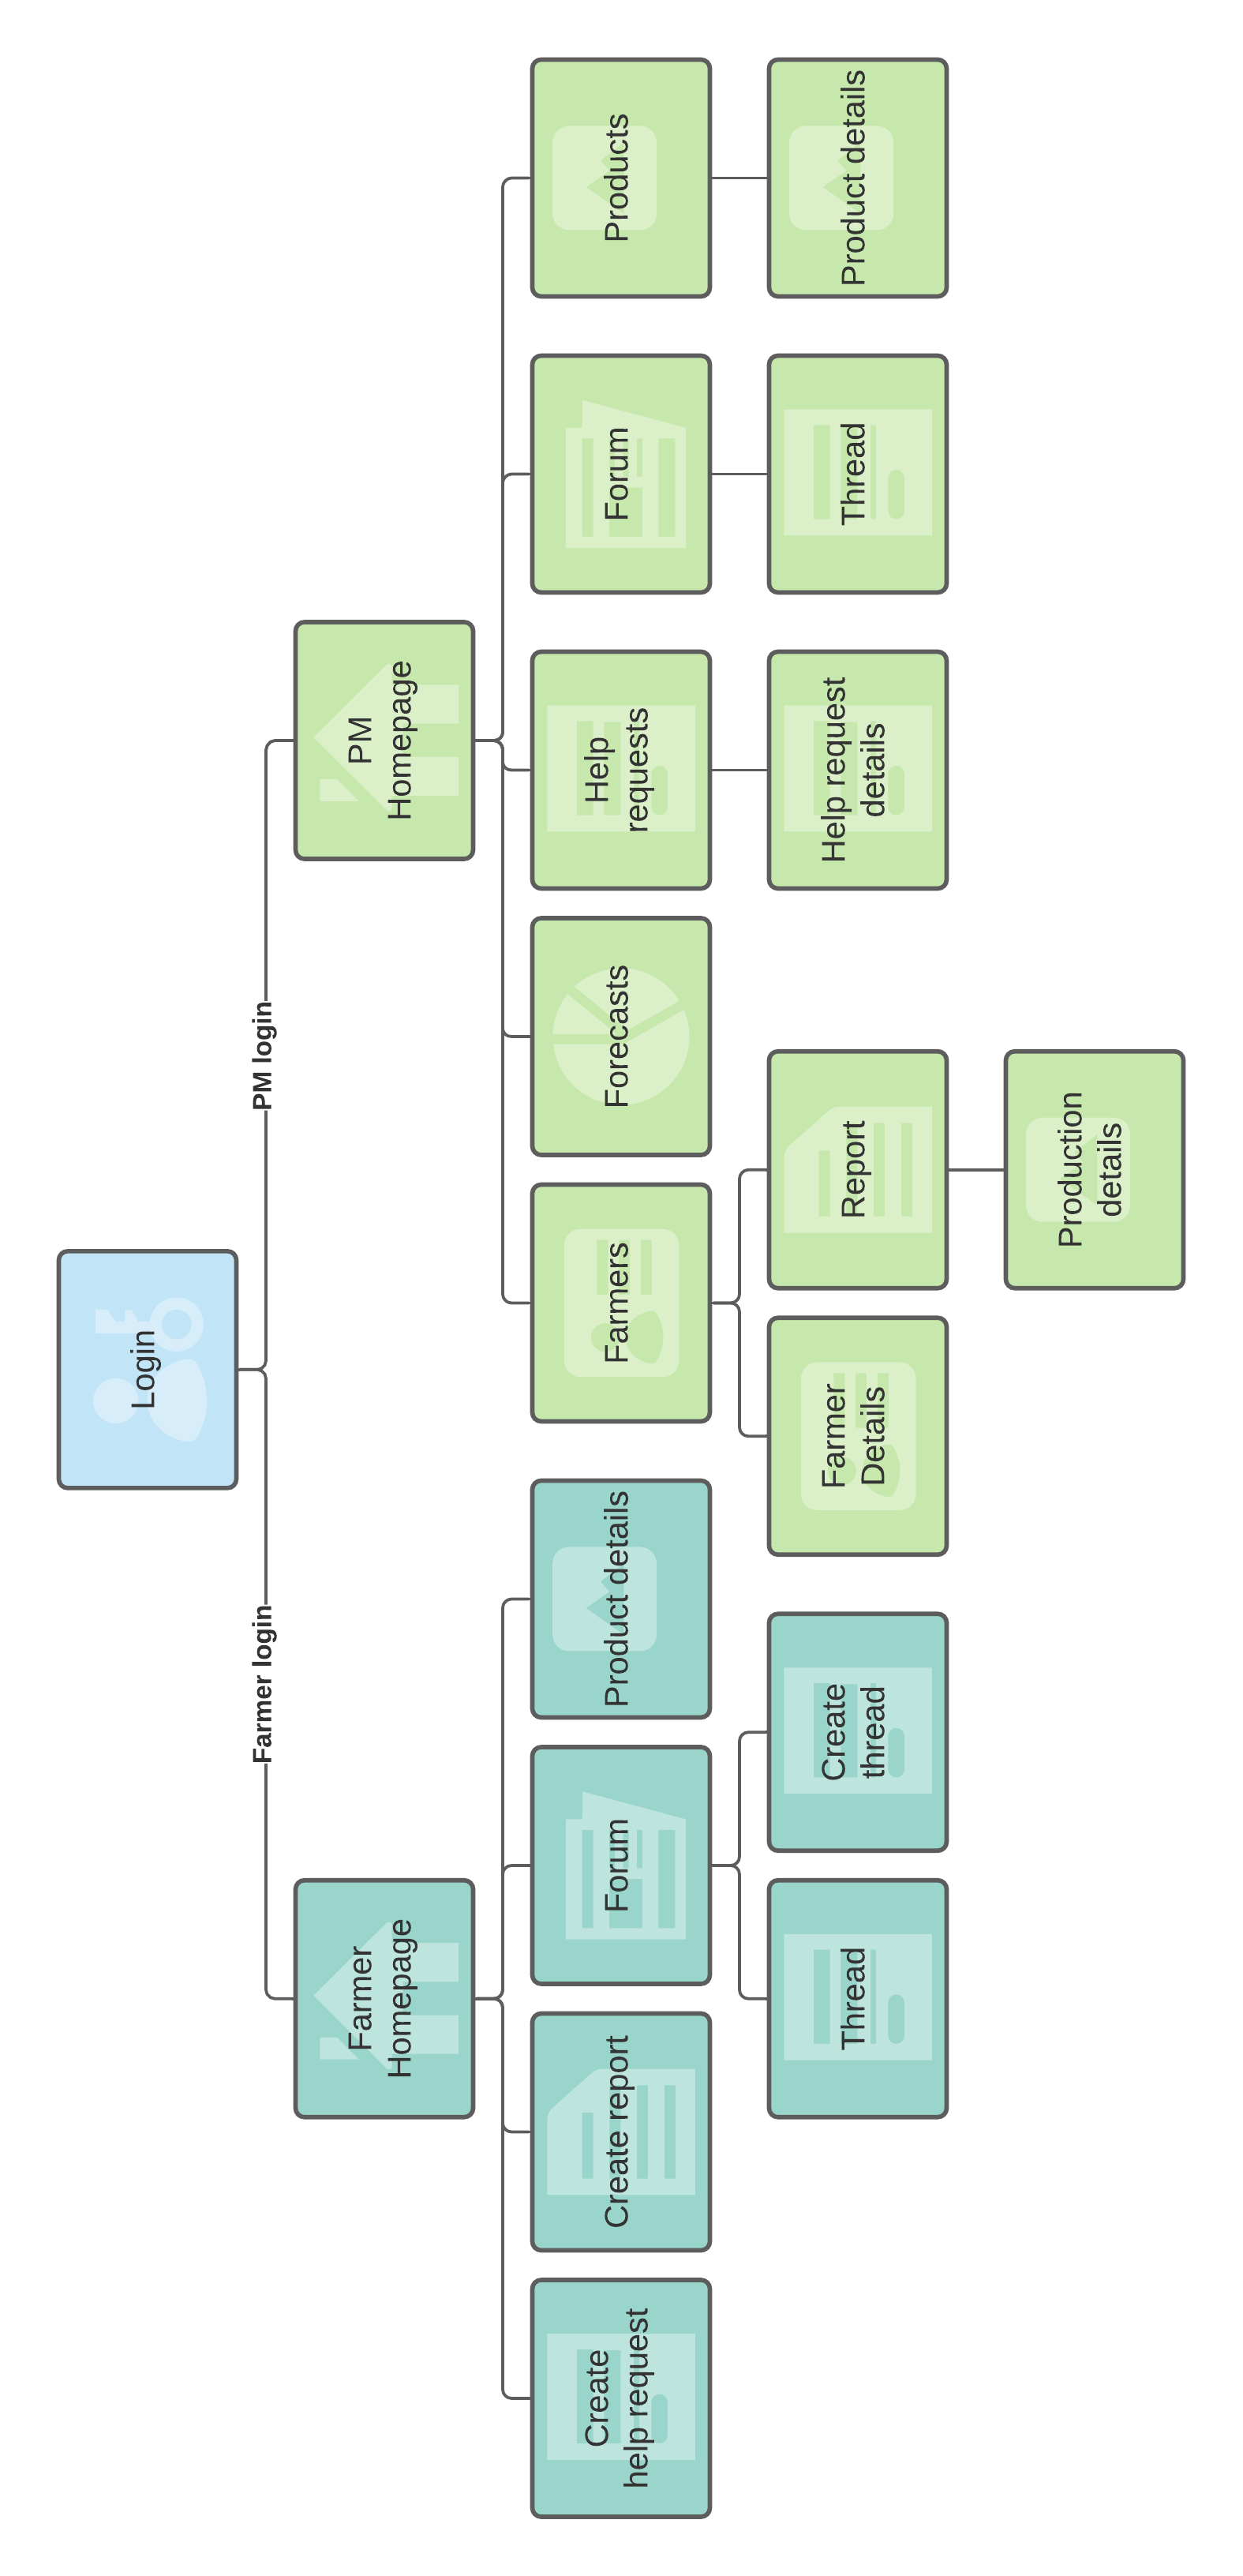
\includegraphics[scale=0.6]{images/uimockups/ui_flow.png}
    \caption{User interface flow}
    \label{fig:ui_flow}
\end{figure}
\section{Requirements Traceability}
This section associates the requirements set forth in the DREAM RASD document with the components designed to meet them.\\
Please note that, for each requirement, only the main components designed to satisfy it have been indicated, in fact the auxiliary components (e.g. Client Handler, Farmer Client, ...) and the sub-components are omitted since they are already described in the previous sections.
\begin{enumerate}[label=\textbf{R\arabic*}]
    \item \label{req:pmReg} The system shall allow system admins to register policy maker.
    \\\textbf{Access Manager, Mail Manager}    
    \item \label{req:pmLogin} The system shall allow policy makers to login. 
    \\\textbf{Access Manager}    
    \item \label{req:farmerReg1} The system shall allow policy makers to register farmers.    
    \\\textbf{Access Manager} 
    \item \label{req:farmerCreds} The system shall provide farmers credentials to log in.    
    \\\textbf{Access Manager, Mail Manager} 
    \item \label{req:farmerReg2} The system shall allow farmers to complete their profile information.    
    \\\textbf{Access Manager} 
    \item \label{req:farmerLogin} The system shall allow farmers to log into the platform.      
    \\\textbf{Access Manager} 
    \item \label{req:farmerReport1} The system shall allow farmers to fill reports with data about goods production.    
    \\\textbf{Report Manager} 
    \item \label{req:farmerReport2} The system shall allow farmers to fill reports with data about auxiliary products used for goods production.    
    \\\textbf{Report Manager} 
    \item \label{req:farmerReport3} The system shall allow farmers to fill reports with problems faced during goods production.     
    \\\textbf{Report Manager} 
    \item \label{req:farmerReport4} The system shall retrieve data from sensors and attach it to reports.     
    \\\textbf{Report Manager, Sensor Manager, Soil Humidity Sensor, Irrigation Sensor} 
    \item \label{req:farmerReport5} The system shall retrieve data from weather stations and attach it to reports.     
    \\\textbf{Report Manager, Weather Manager} 
    \item \label{req:farmerWeather} The system shall allow farmers to visualize weather forecasts.
    \\\textbf{Weather Manager} 
    \item \label{req:farmerSensors} The system shall allow farmers to visualize data retrieved from humidity and irrigation sensors.
    \\\textbf{Sensor Manager, Soil Humidity Sensor, Irrigation Sensor} 
    \item \label{req:farmerForum} The system shall allow farmers to create and contribute to forum discussions.    
    \\\textbf{Forum Manager} 
    \item \label{req:farmerHelp} The system shall allow farmers to create help requests.     
    \\\textbf{Help Request Manager} 
    \item \label{req:farmerSugg} The system shall allow farmers to visualize personalized suggestions about goods and techniques.    
    \\\textbf{Help Request Manager} 
    \item \label{req:pmMonitor} The system shall allow PMs to monitor farmers' performances.    
    \\\textbf{User Manager} 
    \item \label{req:pmParameters} The system shall provide PMs parameters to evaluate farmers' performances.   
    \\\textbf{User Manager} 
    \item \label{req:pmGrades} The system shall allow PMs to compare and aggregate farmers' performances.    
    \\\textbf{User Manager, Dashboard Manager} 
    \item \label{req:pmFilter1} The system shall allow PMs to filter farmers based on their information.    
    \\\textbf{User Manager, Dashboard Manager} 
    \item \label{req:pmFilter2} The system shall allow PMs to filter farmers based on their performance.    
    \\\textbf{User Manager, Dashboard Manager} 
    \item \label{req:pmSort1} The system shall allow PMs to sort farmers based on their information.    
    \\\textbf{User Manager, Dashboard Manager} 
    \item \label{req:pmSort2} The system shall allow PMs to sort farmers based on their performance.     
    \\\textbf{User Manager, Dashboard Manager} 
    \item \label{req:pmRewards} The system shall allow PMs to reward best performing farmers.    
    \\\textbf{User Manager, Dashboard Manager, Mail Manager, Mail Server} 
    \item \label{req:pmWeather} The system shall allow PMs to visualize weather forecasts.    
    \\\textbf{Weather Manager} 
    \item \label{req:pmHelp1} The system shall allow PMs to visualize help requests.
    \\\textbf{Help Request Manager} 
    \item \label{req:pmHelp2} The system shall allow PMs to take charge of help requests.
    \\\textbf{Help Request Manager} 
    \item \label{req:pmHelp3} The system shall allow PMs to visualize farmers who have requested help and their performances.
    \\\textbf{Help Request Manager, User Manager} 
    \item \label{req:pmHelp4} The system shall allow PMs to close help requests.
    \\\textbf{Help Request Manager}
    \item \label{req:pmInterview} The system shall allow PMs to fill reports about farmers interviews.    
    \\\textbf{User Manager}
    \item \label{req:pmVisits} The system shall allow PMs to re-schedule agronommist's control visit plans.    
    \\\textbf{Help Request Manager}
    \item \label{req:pmForum} The system shall allow PMs to create and contribute to forum discussions.    
    \\\textbf{Forum Manager}
    \item \label{req:pmSuggestions} The system shall allow PMs to create suggestions.
    \\\textbf{Help Request Manager}
\end{enumerate}

\section{Implementation, integration and test plan}
\subsection{System Testing}
During implementation, the developed software must be tested step-by-step with unit tests before 
being incorporated into the system. After the entire system has been properly developed and integrated, 
testing of the entire infrastructure will be required to verify its integrity and correctness. 
At this point the test environment should be as close to the production environment as possible, 
the system tests to be performed are:
\begin{itemize}
    \item \textbf{Functional Testing}\\The application is tested to verify that it meets all 
    requirements, i.e., that it is able to function properly under certain conditions. 
    This is a black-box testing methodology, i.e., the internal workings of the tested code 
    are not taken into account, nor are the steps that lead to the result, but only the final result is focused on.\\
    The tool used for this phase must support running scripted test automation, simulating the 
    behavior of farmers and PMs in all scenarios. %selenium per il test scripting 
    \item \textbf{Performance and Load Testing}\\This testing phase is needed to identify bottlenecks affecting response time, utilization,
    throughput and to do benchmarking, in order to establish a baseline thanks to which it will be 
    possible to make comparisons for possible future integrations.\\
    Using the data available to the Telangana Minister of Agriculture, an expected workload will be calculated 
    and acceptable performance will be formulated based on it. The whole system will be under this load, increasing it 
    periodically in order to calculate load treshold and the maximum time the system can be exposed to it. %loadninja
    \item \textbf{Stress Testing}\\After calculating a solid performance baseline, the system will be subjected to 
    loads well beyond expectations to evaluate response and make sure that the system recovers gracefully after failure.
\end{itemize}
\subsection{Testing tools}
\begin{itemize}
    \item \textbf{JUnit}\\Unit testing framework for the Java programming language.
    \item \textbf{TestComplete}\\GUI test automation tool that tests every desktop and web application. Integrates tightly with 
    the tools in your ecosystems, giving you a complete testing lifecycle.
    \item \textbf{LoadNinja}\\LoadNinja allows you to build scriptless load tests. It replaces load emulators with real browsers and generating actionable metrics.
\end{itemize}


\section{Effort spent}

\bibliography{main.bib}

\end{document}